%%% The main file. It contains definitions of basic parameters and includes all other parts.

%% Settings for single-side (simplex) printing
% Margins: left 40mm, right 25mm, top and bottom 25mm
% (but beware, LaTeX adds 1in implicitly)
\documentclass[12pt,a4paper]{report}
\setlength\textwidth{145mm}
\setlength\textheight{247mm}
\setlength\oddsidemargin{15mm}
\setlength\evensidemargin{15mm}
\setlength\topmargin{0mm}
\setlength\headsep{0mm}
\setlength\headheight{0mm}
% \openright makes the following text appear on a right-hand page
\let\openright=\clearpage

%% Settings for two-sided (duplex) printing
% \documentclass[12pt,a4paper,twoside,openright]{report}
% \setlength\textwidth{145mm}
% \setlength\textheight{247mm}
% \setlength\oddsidemargin{14.2mm}
% \setlength\evensidemargin{0mm}
% \setlength\topmargin{0mm}
% \setlength\headsep{0mm}
% \setlength\headheight{0mm}
% \let\openright=\cleardoublepage

%% Generate PDF/A-2u
\usepackage[a-2u]{pdfx}

%% Character encoding: usually latin2, cp1250 or utf8:
\usepackage[utf8]{inputenc}

%% Prefer Latin Modern fonts
\usepackage{lmodern}

%% Further useful packages (included in most LaTeX distributions)
\usepackage{amsmath}        % extensions for typesetting of math
\usepackage{amsfonts}       % math fonts
\usepackage{amsthm}         % theorems, definitions, etc.
\usepackage{bbding}         % various symbols (squares, asterisks, scissors, ...)
\usepackage{bm}             % boldface symbols (\bm)
\usepackage{graphicx}       % embedding of pictures
\usepackage{fancyvrb}       % improved verbatim environment
\usepackage{natbib}         % citation style AUTHOR (YEAR), or AUTHOR [NUMBER]
\usepackage[nottoc]{tocbibind} % makes sure that bibliography and the lists
			    % of figures/tables are included in the table
			    % of contents
\usepackage{dcolumn}        % improved alignment of table columns
\usepackage{booktabs}       % improved horizontal lines in tables
\usepackage{paralist}       % improved enumerate and itemize
\usepackage{xcolor}         % typesetting in color
\usepackage{longtable}		% multipage tables
\usepackage{subfigure}
\usepackage{tikz}
\usepackage{listings}
\usepackage[ruled]{algorithm2e}

% Path to images folder
\graphicspath{ {./images/} }

% Drawing over matrices
\newcommand{\rn}[2]{%% "rn": "remember node"
    \tikz[remember picture,baseline=(#1.base)]\node [inner sep=0] (#1) {$#2$};%
}

%%% Basic information on the thesis

% Thesis title in English (exactly as in the formal assignment)
\def\ThesisTitle{Thesis title}

% Author of the thesis
\def\ThesisAuthor{Name Surname}

% Year when the thesis is submitted
\def\YearSubmitted{YEAR}

% Name of the department or institute, where the work was officially assigned
% (according to the Organizational Structure of MFF UK in English,
% or a full name of a department outside MFF)
\def\Department{Name of the department}

% Is it a department (katedra), or an institute (ústav)?
\def\DeptType{Department}

% Thesis supervisor: name, surname and titles
\def\Supervisor{Supervisor's Name}

% Supervisor's department (again according to Organizational structure of MFF)
\def\SupervisorsDepartment{department}

% Study programme and specialization
\def\StudyProgramme{study programme}
\def\StudyBranch{study branch}

% An optional dedication: you can thank whomever you wish (your supervisor,
% consultant, a person who lent the software, etc.)
\def\Dedication{%
Dedication.
}

% Abstract (recommended length around 80-200 words; this is not a copy of your thesis assignment!)
\def\Abstract{%
Abstract.
}

% 3 to 5 keywords (recommended), each enclosed in curly braces
\def\Keywords{%
{key} {words}
}

%% The hyperref package for clickable links in PDF and also for storing
%% metadata to PDF (including the table of contents).
%% Most settings are pre-set by the pdfx package.
\hypersetup{unicode}
\hypersetup{breaklinks=true}

% Definitions of macros (see description inside)
%%% This file contains definitions of various useful macros and environments %%%
%%% Please add more macros here instead of cluttering other files with them. %%%

%%% Minor tweaks of style

% These macros employ a little dirty trick to convince LaTeX to typeset
% chapter headings sanely, without lots of empty space above them.
% Feel free to ignore.
\makeatletter
\def\@makechapterhead#1{
  {\parindent \z@ \raggedright \normalfont
   \Huge\bfseries \thechapter. #1
   \par\nobreak
   \vskip 20\p@
}}
\def\@makeschapterhead#1{
  {\parindent \z@ \raggedright \normalfont
   \Huge\bfseries #1
   \par\nobreak
   \vskip 20\p@
}}
\makeatother

% This macro defines a chapter, which is not numbered, but is included
% in the table of contents.
\def\chapwithtoc#1{
\chapter*{#1}
\addcontentsline{toc}{chapter}{#1}
}

% Draw black "slugs" whenever a line overflows, so that we can spot it easily.
\overfullrule=1mm

%%% Macros for definitions, theorems, claims, examples, ... (requires amsthm package)

\theoremstyle{plain}
\newtheorem{thm}{Theorem}
\newtheorem{lemma}[thm]{Lemma}
\newtheorem{claim}[thm]{Claim}

\theoremstyle{plain}
\newtheorem{defn}{Definition}

\theoremstyle{remark}
\newtheorem*{cor}{Corollary}
\newtheorem*{rem}{Remark}
\newtheorem*{example}{Example}

%%% An environment for proofs

\newenvironment{myproof}{
  \par\medskip\noindent
  \textit{Proof}.
}{
\newline
\rightline{$\qedsymbol$}
}

%%% An environment for typesetting of program code and input/output
%%% of programs. (Requires the fancyvrb package -- fancy verbatim.)

\DefineVerbatimEnvironment{code}{Verbatim}{fontsize=\small, frame=single}

%%% The field of all real and natural numbers
\newcommand{\R}{\mathbb{R}}
\newcommand{\N}{\mathbb{N}}

%%% Useful operators for statistics and probability
\DeclareMathOperator{\pr}{\textsf{P}}
\DeclareMathOperator{\E}{\textsf{E}\,}
\DeclareMathOperator{\var}{\textrm{var}}
\DeclareMathOperator{\sd}{\textrm{sd}}

%%% Transposition of a vector/matrix
\newcommand{\T}[1]{#1^\top}

%%% Various math goodies
\newcommand{\goto}{\rightarrow}
\newcommand{\gotop}{\stackrel{P}{\longrightarrow}}
\newcommand{\maon}[1]{o(n^{#1})}
\newcommand{\abs}[1]{\left|{#1}\right|}
\newcommand{\dint}{\int_0^\tau\!\!\int_0^\tau}
\newcommand{\isqr}[1]{\frac{1}{\sqrt{#1}}}

%%% Various table goodies
\newcommand{\pulrad}[1]{\raisebox{1.5ex}[0pt]{#1}}
\newcommand{\mc}[1]{\multicolumn{1}{c}{#1}}


% Title page and various mandatory informational pages
\begin{document}
%%% Title page of the thesis and other mandatory pages

%%% Title page of the thesis

\pagestyle{empty}
\hypersetup{pageanchor=false}
\begin{center}

\centerline{\mbox{
\includegraphics[width=166mm]{./logo-en.pdf}}}

\vspace{-8mm}
\vfill

{\bf\Large BACHELOR THESIS}

\vfill

{\LARGE\ThesisAuthor}

\vspace{15mm}

{\LARGE\bfseries\ThesisTitle}

\vfill

\Department

\vfill

{
\centerline{\vbox{\halign{\hbox to 0.45\hsize{\hfil #}&\hskip 0.5em\parbox[t]{0.45\hsize}{\raggedright #}\cr
Supervisor of the bachelor thesis:&\Supervisor \cr
\noalign{\vspace{2mm}}
Study programme:&\StudyProgramme \cr
\noalign{\vspace{2mm}}
Study branch:&\StudyBranch \cr
}}}}

\vfill

% Zde doplňte rok
Prague \YearSubmitted

\end{center}

\newpage

%%% Here should be a bound sheet included -- a signed copy of the "bachelor
%%% thesis assignment". This assignment is NOT a part of the electronic
%%% version of the thesis. DO NOT SCAN.

%%% A page with a solemn declaration to the bachelor thesis

\openright
\hypersetup{pageanchor=true}
\pagestyle{plain}
\pagenumbering{roman}
\vglue 0pt plus 1fill

\noindent
I declare that I carried out this bachelor thesis independently, and only with the cited
sources, literature and other professional sources. It has not been used to obtain another
or the same degree.

\medskip\noindent
I understand that my work relates to the rights and obligations under the Act No.~121/2000 Sb.,
the Copyright Act, as amended, in particular the fact that the Charles
University has the right to conclude a license agreement on the use of this
work as a school work pursuant to Section 60 subsection 1 of the Copyright~Act.

\vspace{10mm}

\hbox{\hbox to 0.5\hsize{%
In \hbox to 6em{\dotfill} date \hbox to 6em{\dotfill}
\hss}\hbox to 0.5\hsize{\dotfill\quad}}
\smallskip
\hbox{\hbox to 0.5\hsize{}\hbox to 0.5\hsize{\hfil Author's signature\hfil}}

\vspace{20mm}
\newpage

%%% Dedication

\openright

\noindent
\Dedication

\newpage

%%% Mandatory information page of the thesis

\openright

\vbox to 0.5\vsize{
\setlength\parindent{0mm}
\setlength\parskip{5mm}

Title:
\ThesisTitle

Author:
\ThesisAuthor

\DeptType:
\Department

Supervisor:
\Supervisor, \SupervisorsDepartment

Abstract:
\Abstract

Keywords:
\Keywords

\vss}

\newpage

\openright
\pagestyle{plain}
\pagenumbering{arabic}
\setcounter{page}{1}


%%% A page with automatically generated table of contents of the bachelor thesis

\tableofcontents

%%% Each chapter is kept in a separate file
\chapter*{Introduction}
\addcontentsline{toc}{chapter}{Introduction}

% his speech does not  flow in a natural way - nie je pravda , je to naopak
Imagine, for a moment, that you are transported in time to 10th-century Europe. It is Sunday, and the weekly mass is just
starting. Look around yourself. The tall ceilings of the impressive church were built so to bring you closer to God. The stained glass windows
let through just enough light so that it is not completely dark. Can you smell the incense? Everything in the environment around
you reminds you that you are taking part in a sacred ritual. Listen to the priest; when he recites the prayers, his speech does not 
flow in a natural way. Instead, the entire text is intoned on a single note, except for the slightly inflected ends of clauses. 
Sometimes, the choir replaces the priest, singing more elaborate monophonic melodies. The words they are singing are Latin, but even 
if you do not understand them, you know what their purpose is: to celebrate the deity. Their voices echo in the stone church, creating an
otherwordly experience.

What you are hearing is called emph{Gregorian chant}, one of the oldest preserved types of music. It has been central to the cultural development
of most of Europe, as it is a part of the Roman-catholic tradition. Figure \ref{fig:chant_manuscripts} shows an example of four chants
\footnote{\url{http://www.ksbm.oeaw.ac.at/images/AT/5000/AT5000-1011/AT5000-1011\_1v.jpg}}\footnote{\url{http://www.uni-regensburg.de/Fakultaeten/phil\_Fak\_I/Musikwissenschaft/cantus/microfilm/copenhagen/vol3/images/008.jpg}}\footnote{\url{http://manuscripta.at/diglit/AT5000-589/09}}\footnote{\url{https://gallica.bnf.fr/ark:/12148/btv1b10033588d/f5.image}} as they are found in
the original manuscripts. The chant in the upper right corner uses notation which is not dissimilar from contemporary musical notation,
while the chant in the lower right image only uses memory aids without the exact pitch. This highlights the differences
between the ways chant was recorded over the centuries (see Section \ref{section:notation}).

\begin{figure}[h]
\centering
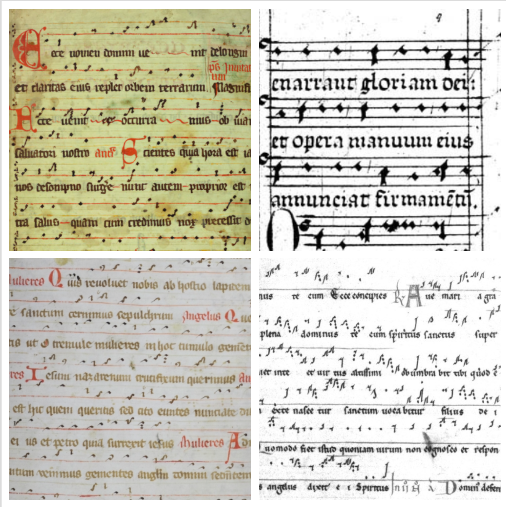
\includegraphics{chant_manuscripts}
\caption{An example of chants as inscribed in manuscripts.}
\label{fig:chant_manuscripts}
\end{figure}

Gregorian chant is a widely researched topic of study, partly thanks to the substantial amount of available sources. However, traditional
musicology is limited by the individual capacity; it is infeasible to study extremely large numbers of chants by hand. This is where
Digital Humanities come into play. Digitalization of large corpora of Gregorian chant enables researchers to draw conclusions
supported by much more data than a human could ever examine.

Nevertheless, contemporary Gregorian chant research still lacks software tools that would facilitate the study of chant repertoire. An example
of an important problem is chant's historical and geographical development. Throughout the 
centuries, the tradition spread accross Europe, while always changing a small part of it. This has led to many variations of the same
chants existing at the same time. Knowing how exactly the changes came into place could shed light on many open questions in the history of 
European culture.

\textbf{The aim of this thesis is to create a tool that musicologists could use to answer questions about chant origin and evolution.} We do this by employing
well-known algorithms for multiple sequence alignment from bioinformatics. Once the idea is proposed, it is almost immediately obvious that
biological and musical sequences share features which warrant using the same methods on both. As opposed to other sequence comparison techniques, such as edit
distance, MSA algorithms do not need any assumptions about the length of chants or other characteristics, which is why they are suitable
for the study of chant.

% screenshot alignmentu s conservation profilom

The tool provides the ability to align a set of chants that is potentially large and diverse in multiple ways, each of which has slightly different uses. One important
implication of the tool is that it makes the discovery contrafacta (chants with the same melody but different lyrics) and transpositions
(chants with the same melody but shifted by an interval) across large repertoires easy.

It is important to note that the purpose of this thesis is not to conduct experiments. It is merely a tool for musicologists who possess
the knowledge needed to select the appropriate data so that previously infeasible discoveries can be made.


\chapter{Related work}

With the advent of computers, the field of Music Information Retrieval (MIR) emerged. Research in this interdisciplinary field focuses on extracting
information from musical notation using computer science methods, such as signal processing or machine learning. Its applications
vary widely, from recommender systems, to automatic audio transcription, to music generation. MIR encompasses all different kinds of music,
regardless of their location, age, or function. Researchers have developed a multitude of software tools that facilitate music analysis,
irrespective of what type of music it is. One of such toolkits is \emph{music21} \citep{music21}, a Python package able to encode musical notation
as Python objects and perform analysis on large datasets.

The study of plainchant using computational methods has not been done extensively. The main research tool for musicologists in this field
is the Cantus Index \citep{cantus_index}. It is an online index of chants from several different chant databases, providing researchers with 
a common API for all of them. The entries in Cantus Index only contain four data fields: full-text, genre, feast (not required), and Cantus ID,
which is automatically assigned to newly added chants. The tool is also able to search for melodies in the original source and even provides 
search-by-melody functionality. There are ten databases indexed in the catalogue, the largest of which is the Cantus database \citep{cantus_db}.

\cite{chant21} developed \emph{chant21}, a Python package able to convert two standard melodic notations, \emph{volpiano} and \emph{gabc} to
a \emph{music21} object, therefore making it easier to study Gregorian chant computationally. The data they used were 
scraped from Cantus database \citep{cantus_db} and GregoBase \citep{gregobase} and released as CantusCorpus and GregoBaseCorpus, respectively.
Finally, they performed two case studies using the package. In the first one, they confirmed the melodic arch hypothesis \citep{melodic_arch}, 
which had previously only been studied manually. Second, they analyzed the relation between differentiæ and antiphon openings \citep{differentiae}
and found that it differs accross modes.

Some of the computational research into plainchant has been centered on mode classification. \cite{mode_huron} used pitch class profiles to
classify modes. They created a pitch-class distribution for each of the eight modes, and used these classes to classify previously unseen data.
\cite{mode_cornelissen} compared three approaches to mode classification: classical approach, which classifies chants based on
the final pitch, range, and the initial pitch; profile approach, which was largely inspired by \cite{mode_huron}; and distributional approach,
which focuses on the melodic aspect of mode. The authors chose various segmentations and representations of chants and used a tf-idf vector
model to classify mode. The study found that we can accurately classify mode even when we discard all absolute pitch information, the melody
contour contains enough information on its own.

A considerable amount of research has been done into the evaluation of melodic similarity, albeit not for Gregorian chant specifically.
\cite{melodic_similarity} provides an overview of the methods. He mentions edit distance, Markov chains, and geometric measurements as
the most widely used ones. \cite{similarity_plot} used an adapted edit distance metric to calculate the similarity of two melodic sequences
by first calculating the similarity for all segments of each of the sequences and then scaling them by a weight function depending on the
segment length, which yielded them what they call a multi-scale similarity stack. The overall similarity was obtained by averaging its values.
Then they used the MSS stack to create a visualization that takes on the shape of a trapezoid that shows which segments of two sequences
are the most similar.

\cite{similarity_bioinf} argue that methods originally developed for bioinformatics have a great potential to be applied to music. They offer
analogies for bioinformatics concepts found in musicology. For example, they liken DNA and proteins to melodic sequences, homologues (proteins that
have the same ancestor) to song covers, evolution to oral transmission, etc. They claim that despite the similarities, MRI has not leveraged the
full potential of bioinformatics methods. In their article, they focus on modelling melodic similarity using multiple-sequence alignment (MSA)
algorithms, therefore not relying on heuristics, as opposed to previous works. Their results revealed that the MAFFT algorithm yields the best
alignemnt, which can be attributed to the algorithm using gap-free segments as anchor points, therefore partitioning melodies into more meaningful
segments than other algorithms.

The general algorithm for calculating pairwise sequence alignment is the Needleman-Wunsch algorithm \citep{needleman}. It uses dynamic programming
to break down the problem into smaller problems. Given two sequences, it starts aligning them from the beginning. At each point, the algorithm checks
whether the two sequences match in the current position, and if not, whether it will leave the elements mismatched or insert a space. In essence,
all possible alignments are computed and scored and the best one is chosen. The algorithm always yields an optimal alignment, therefore it is
used when the quality of the alignment is important. However, because of its time complexity, it is unsuitable for many applications.

Unlike pairwise sequence alignment, multiple sequence alignment has been shown to be NP-complete \citep{msa_complexity}. As such, there is no practical
way of computing an optimal MSA and we must instead rely on heuristics to obtain a sufficiently good alignment.

\cite{msa_overview} provides an overview of modern multiple sequence alignment algorithms. According to him, the most frequently used algorithms use
the progressive approach, where a guide tree is estimated from unaligned sequences and then pairwise alignment algorithms are used to find
the MSA following the tree. He notes that the scoring methods of the pairwise algorithm are essential. There are two main groups of scoring methods:
matrix-based algorithms, where a substitution matrix is used to determine the cost of replacing one symbol with another, and the consistency-based
methods, which use a collection of global and local alignments to calculate a position-specific substitution matrix. The author claims that
the best methods yield indistinguishable results, except for remote homologs with less than 25\% identity.

T-Coffee \citep{t_coffee} uses the progressive approach described above. It was the first algorithm that used a preprocessed collection of 
alignments to create a library that helps create the guide tree. The library is generated using both global and local pairwise alignments.
Thanks to this approach, T-Coffee minimizes the errors made in the first stages of building the MSA, which is a shortcoming of many previous
algorithms, as these errors tend to persist. They combined precomputed local and global alignments and create a function that assigns a weight to
each pairwise alignment depending on how consistent the pair of residues is with the residue pairs from all other alignments. This process
leads to a significant improvement of the results.

MAFFT \citep{mafft} further improves on other methods by using Fast Fourier transform to identify homologues fast. In addition, the authors
propose a simplified scoring system that reduces CPU time while maintaining its accuracy. The authors' results showed a performance 
100 times better than that of T-Coffee. 

Despite the fact that MSA algorithms have already been used for music analysis, this is the first work that focuses specifically on applying
the methods on Gregorian chant. Gregorian chant is specific by its monophonic nature, which means that there is just one sequence to analyze.
Each chant has also undergone many changes over the centuries, therefore there are many variants of the same chants that can be
researched. These characteristics make Gregorian chant an ideal subject for MSA analysis and subsequent application of related bioinformatics methods.

% one sequence to analyze (as is the case of modern repertoire)

\chapter{Gregorian chant}

\emph{This chapter is adapted after \cite{chant_book}.}

In order to design an application that processes chant data, it is necessary to understand the basics of what Gregorian chant is.

Gregorian chant is the music associated with the Roman catholic tradition. It is sung in churches, as well as in convents, and can also be sung during outdoor
ceremonies such as processionals (and outdoor liturgy in general.). Its current written form is, as far as we can tell, very similar to its original
form from the first millenium.

Gregorian chant is one of the earliest forms of music preserved in written form, and the
largest preserved body of medieval music. The earliest preserved fragments of written notes date back to the 9th century, although texts from as early as 
the eighth century have been found.. Its name, Gregorian, references Pope Gregory the Great, however, his relation to the chant is not entirely clear.

It is not the only type of chant. In the early centuries after Christianity spread across Western and Eastern Roman Empire,
new forms of worship started being developed. The most obvious differences were between the West and the East, which had multiple cultural
centers such as Constantinople, Jerusalem, or Alexandria. However, liturgies varied in the West as well, from Rome to Milan to the Iberian peninsula to Gaul.
Each center developed their own tradition, including their own type of chant. Roman-catholic tradition being so prevalent in Europe
can be attributed to Charlemagne's attempt to unify European kingdoms.

Gregorian chant is an integral part of the Roman church, and has been so for centuries. It is the monophonic music (i.e. single-voice)
sung during liturgy at specific points, defined by the rules for conducting liturgy according to the Roman rite (the rite of the Latin church, or what
we know as the Catholic church today). Here, liturgy means chant sung during Christian worship. Unlike in the Eastern churches, where the term is reserved 
for the Eucharist, liturgy includes both the Mass and the Divine Office in the Roman church.

As with other kinds of music, there exist several genres of Gregorian chant. A \emph{genre} is a group of chants that share some characteristics, such as
complexity or content. Different genres play different roles in the liturgy. Some are sung while the priest is walking to the altar, others convey the
core message of a mass, others have just a decorative purpose.

Not all genres are sung during every kind of worship. In the following section, we describe the Mass and the Divine Office and mention some genres
that are specific for each.

\section{Mass and Divine Office}

Mass is the service most familiar to most believers.
It can be divided into several parts, all leading up to the most important one, the act of communion. This act commemorates the Last Supper,
Jesus's last meal with his disciples before his execution. During the communion, bread, representing Christ's body, and wine, representing his
blood, are given out. During the course of the Mass, multiple different chants are sung. \emph{Introitus}, meaning 'entrance', is sung at the beginning
of the service while the priest and his assistants are walking to the altar. \emph{Tractus} is a chant that is sung during Lent, i.e. the period
between Ash Wednesday and the Saturday before Easter. Outside of this period, \emph{alleluia} replaces \emph{tractus} and is followed by \emph{sequentia}
on the most important feast days.

The other part of the liturgy, besides the Mass, is the Divine Office, also called Liturgy of the Hours or canonical hours. It is the set of chants
sung during services at different times of the day, for example \emph{Vespers} in the evening or \emph{Lauds} in the morning. The office consists
largely of singing psalms, of which there are 150, all sung on different days and hours. Psalms were usually preceded and followed by antiphons,
which differ not only by the day of the week, but also depending on the position within the liturgical year. Each day of the week had an allocated
set of antiphons, hymns and responsories, while responsories were assigned to the different Sundays. Additionally, important feasts had their own
set of chants to be sung.

The liturgical year consists of many feasts. Some feasts are fixed on a specific date. Feasts associated with a specific saint are an example of those.
For example, John the Baptist is celebrated on the 24th of June, Michael on the 29th of September, and All Saints on the 1st of November. Other
fixed-date feasts include Christmas Day (25 December), Epiphany (6 January), and others. Such feasts can fall on any day of the week, and if they fall
on a Sunday, they will take precedence over it. On the other hand, there are also feasts that are fixed to a specific day of the week, the most important
of them being Easter Sunday, the day when Christ rose from the dead. Each feast has a different set of chants that can be completely original.

\section{Variation between chants}

The individual chants differ in several criteria, the first one being the \emph{mode}. Mode is the system of pitch organization, somewhat similar to modern-day
scales. All chants use the seven tones of a diatonic scale, meaning a scale with five whole steps and two half steps.

Melodies are classified into one of eight modes according to their last note, called \emph{finalis}, and their range. Most chants
end on one of the notes \emph{D}, \emph{E}, \emph{F}, or \emph{G}. These four notes determine four pairs of modes. The melodies were further classified
depending on whether they moved mostly in the range above the \emph{finalis}, in which case it would be classified as the \emph{authentic} mode
of the pair, or in the range around the \emph{finalis}, which means it is classified as the \emph{plagal} mode. Some types of chant tend to
occur mostly in a specific mode.

\begin{figure}[h]
\centering
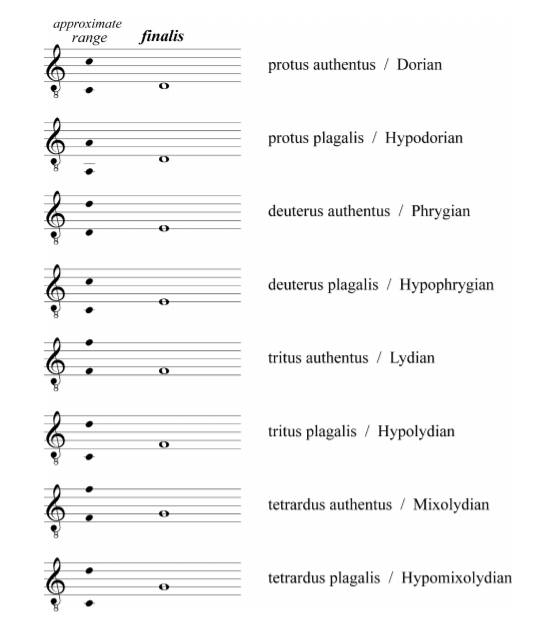
\includegraphics[scale=0.7]{modes}
\caption{List of modes, their ranges and finalis. \cite[p.~44]{chant_book}}
\end{figure}

Another criterion is the complexity of chants, that is, how elaborate the melody is. On the one side of the spectrum, there is a one-to-one
syllable to note correspondence. Antiphons and some hymns are genres close to this text-setting. The other extreme is melismatic style. Melisma
is a long vocalization of a single syllable, therefore melismatic melodies are more ornate. Some of the more melismatic genres are the gradual,
tract and offertory.

We have already mentioned several different genres of chant. Antiphons are chants sung to frame a psalm during the Office hours. They are relatively
short and simple, somtimes consisting of only two phrases. Responsories are sung during the Night Office. Each has a main section and a verse. They are
melodically very rich and are on of the most impressive forms of chant. The number of chants sung during the Mass is lower, as there will usually
only be one introit, one gradual, etc. during a service.

It is important to note that text and melody do not form unique pairs. Instead, each text
can be sung to multiple different melodies and multiple texts can be sung to one melody. Chants with the same melody but different lyrics
are called \emph{contrafacta}.

\section{Chant notation}
\label{section:notation}

It is clear that the annual cycle is very complex and the amount of chants is abundant. Therefore, it is not surprising that while the chants during the
services themselves were sung from memory, they were written down in books. Each church and each convent had their own manuscripts, which is the
reason of their abundance.

At first, melodies were written without a staff. The writers simply marked the direction in which the pitch was moving, serving barely as memory aids,
not for learning. Later, better accuracy was required,
therefore melodies started being written with their exact pitch, resembling the modern-day musical notation. However, written melodies never contained
explicit information about the rhythm. An example of a chant melody as found in a manuscript is shown in Figure \ref{fig:chant}.

\begin{figure}[h]
\centering
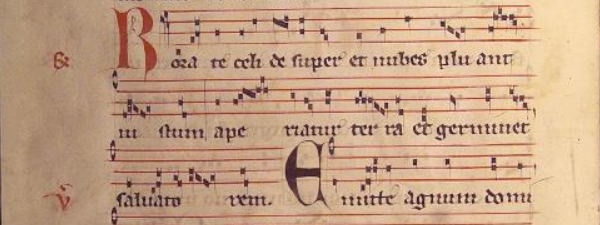
\includegraphics{manuscript}
\caption{Example of a chant in a manuscript. \cite[id~007553]{cantus_db}}
\label{fig:chant}
\end{figure}

In the middle ages, tools to tune singers' voice to a specific pitch were not readily available. This led to the singing ``by feeling''. As a result,
some churches or convents sang the same melody, but shifted by a certain interval, and they were inscribed in manuscripts with this shift. Such melodies
(those that differ by the same interval in all positions) are called \emph{transpositions}.

\section{Digital chant research}

The study of Gregorian chant is an active area of musicology covering many centuries and the whole continent. It has a rich digital infrastructure facilitating
the research using computational methods. There exist several large databases of digitalized chants, such as the Cantus database\footnote{\url{https://cantus.uwaterloo.ca/}},
and the databases are indexed in the Cantus Index,\footnote{\url{http://cantusindex.org/}}, providing a standard API for searching among them.

There are several problems that can be tackled using computational methods. For example, some researchers have a sense that women's houses may have used
transposed modes more frequently than men's houses. However, no research has been done on this topic yet, as it requires comparing too many chants to draw
a conclusion with reasonable scientific certainty. Computational methods could help quantify the numbers.
Another question is whether mode distribution is different according to monastic order. It is also possible to find if there is a regional preference for
pitch progression (e.g. A-B-A vs. A-C-A) by comparing manuscripts.\footnote{From personal communication with Debra Lacoste and Jennifer Bain.}

These are examples of problems that have not been properly researched yet, but the digitalization of resources makes the research feasible.

\chapter{Data}

Our main source of data is the Cantus database (\cite{cantus_db}), one of the databases indexed in the Cantus Index. The database serves as a 
digital archive of chants, each entry containing information about its source, liturgical occasion, mode, and others. Work on the project started
in the late 1980s, and to date, around 500,000 individual chants from approximately 150 manuscripts have been indexed. Each entry is transcribed 
manually and undergoes a thorough examination before publishing (\cite{cantus_lacoste}).

We are using a scraped version of the Cantus database released as CantusCorpus (\cite(chant21)). Unlike the Cantus database which is continuously being
updated and is therefore unsuitable for computational study, the corpus is versioned, therefore each version always contains the same data. We are using
version 0.2 released in July 2020 which contains 497071 entries. The corpus is available for download in CSV format.

\section{CSV}

CSV is one of the most common formats for tabular data. The abbreviation stands for \emph{comma-separated values}. As the name suggests, the format
uses commas to separate columns (although other separators, such as a semicolon, can be used as well to allow for simpler parsing in case that the data 
frequently contains commas that would otherwise need to be escaped), while the individual rows are separated by a line break. The data is stored as plaintext,
which makes it easily readable. Parsing CSV files becomes more complicated when the data contains column and row separators inside fields; in that case
quotation marks or esape sign has to be used. There exist many well-designed parsers, one such parser is the Python module simply called \emph{CSV}.

\section{Database fields}

The csv files in Cantus Corpus contain 21 fields (excluding its row number), of which we are only using a subset.

Each entry contains the chant's incipit, which is the first few words of the text. As chants do not have a title, incipit can substitute its role
in contexts where one is needed.

The fields position, sequence, and folio represent the exact location of the original chant in a manuscript from which it was transcribed.

feastid represents the liturgical occasion when the chant was intended to be performed, or, in other words, a feast. Similarly, officeid represents
the liturgical time of the day during which it was sung.

The text and melody of the chant are found in the fulltext and volpiano fields, respectively. Entries can contain both, either, or none of these fields.

\section{Volpiano}

The melodies in the volpiano fields are encoded as strings of alphanumeric characters and dashes. These can be rendered as musical notation using
the volpiano font. Each character represents either a pitch, empty space, or other musical characters, such as a clef.

Volpiano was developed as a research tool optimized for databases and word processors. There are strict rules concerning the transcription, which leads
to all volpiano-encoded melodies having a standardized format. Each transcription begins with a treble clef. Gaps between words are encoded as three
dashes, while two dashes represent gaps between syllables (\cite{volpiano}).


\chapter{Multiple sequence alignment}

Sequence alignment, in general, is a task whose purpose is to arrange two or more sequences with a common alphabet to identify similar
and different regions within them. A set of sequences being \emph{aligned} in this case can be understood as each being extended by spaces
in such a way that if they are arranged in a matrix, each sequence occupying one row and each column containing one character, it can be seen
what had to happen for one sequence to change into another on a character-by-character basis: insertion (or deletion), character substitution,
or nothing if the characters in the given position are identical. A good sequence alignment algorithm is one that does not perform
unnecessary insertions (deletions) or substitutions.

The problem of multiple sequence alignment is most studied in bioinformatics. Since DNA was first sequenced
in the 1970s, there has been a need to compare various genomes to determine similarity. As organisms mutate and evolve, their
DNA or RNA changes. Aligning their genomes reveals similar and different regions, which facilitates the tracking of these
mutations and makes it possible to determine the order in which they happened.

However, the applications of sequence alignment are not limited to biology. Every task that makes use of determinig the similarity
of some sequences, where the emphasis is put on finding regions where they do not diverge, can make use of the existing methods.

Melody alignment of Gregorian chant can be considered as such. As the tradition spread across Europe, each place changed some of 
the existing melodies by a little, thereby creating new melodies that can change further as they travel through time and space.
This is akin to the mutations in DNA caused by environmental factors. Finding well-conserved regions in many instances of chant
provides great insight into which parts of a melody are unlikely to change, and, on the other hand, which ones tend to vary
a lot. It can also reveal the ancestors of a melody and the path which it traveled to transform into its final form.
This is in line with the focus of philology shifting not to merely reconstructing an earliest layer of a text (with the unspoken 
assumption that this is the ``real'' text), but to map the entire tradition of text transmission and evolution, taking the later layers 
to be as valid within their cultural environment as the older layers.


In this chapter, we will first give the definition of the problem of sequence alignment. We will mention some important considerations,
as well as theoretical limitations. Then we will provide an overview of the methods developed for bioinformatics that attempt to solve
the problem. Finally, we will show how we applied the existing methods and technologies on Gregorian chant melodies.

\section{The problem of sequence alignment}

Assume that we have an alphabet $\mathcal{A}$ and a character $\sigma$ such that $\sigma \notin \mathcal{A}$. Then let us have a set
of sequences $S = \{s_1, s_2, ..., s_k\}$ with $s_i \in \mathcal{A}^{l_i}$. The output of a sequence alignment algorithm is the set of
aligned sequences $A = \{a_1, a_2, ..., a_k\}$, where $a_k \in (\mathcal{A}\cup\{\sigma\})^L$, $L \geq l_i \:\forall i\in\{1, 2, ..., k\}$.
Each original sequence $s_i$ can be obtained from the aligned sequence $a_i$ by removing all $\sigma$.

Given two aligned sequences $a_i$ and $a_j$ and an index $p \leq L$, we define the following operations:

\begin{itemize}
    \item \emph{Identity}: $(a_i)_k = (a_j)_k$
    \item \emph{Insertion}: $(a_i)_k = \sigma \land (a_j)_k \in \mathcal{A}$
    \item \emph{Deletion}: $(a_i)_k \in \mathcal{A} \land (a_j)_k = \sigma$
    \item \emph{Substitution}: $(a_i)_k \in \mathcal{A} \land (a_j)_k \in \mathcal{A} \land (a_i)_k \neq (a_j)_k$
\end{itemize}

Each of the operations has an associated cost. The cost of substitution can further vary depending on which characters are being
substituted. We can then define the overall cost of the alignment $A$ in different ways, e.g. as the sum of costs over all triples
$(i, j, p) \: \forall i, j \in \{1, 2, ..., k\} \: \forall p \leq L$ or as the sum of costs for unordered pairs $\{i, j\}$ and indices $p$,
in which case insertion and deletion are considered the same operation. The goal of a sequence alignment algorithm is to minimize the cost.
There are other, more complicated ways of defining the cost  function, and the performance of an algorithm is highly dependent on which one it uses.

\subsection{Pairwise and multiple sequence alignment}

Depending on the number of sequences to align, we distinguish between pairwise alignment for pairs of sequences and multiple sequence alignment
for more than two. Despite the similarity in their outcomes, the two problems are fundamentally different from a computational perspective.

Pairwise alignment is relatively easy to solve. The Needleman-Wunsch algorithm, which is a dynamic programming algorithm, can find an optimal
solution in the asymptotic time of $\mathcal{O}(mn)$, where $m$ and $n$ are the respective lengths of the sequences. This means that it is
possible to find an optimal alignment even for longer sequences.

Needleman-Wunsch algorithm can be extended to more than two sequences. However, with each additional sequence, its complexity increases,
and it quickly becomes impractical or even practically impossible to align multiple sequences this way. In fact, it has been proven that multiple sequence
alignment is an NP-complete problem \citep{msa_complexity}. It is therefore necessary to use various heuristics to generate alignments. Current
algorithms do not aim at finding the optimal alignment; instead, they try to produce one that is good enough.

\subsection{Local and global sequence alignment}

There is a distinction to be made between local and global sequence alignment.

The problem description above is the definition of global alignment. Aligning sequences globally means aligning the entire sequences end-to-end.
(This does not mean, however, that there cannot be gaps at the beginning or at the end of the generated alignment.)
All characters from all sequences must be present in the final alignment. Global alignment is used to compare relatively similar
sequences, such as protein homologues or versions of the same chant sung at different points in time.

On the other hand, the goal of local alignment is to find similar regions in divergent sequences, while the rest of the sequences is disregarded.
The output of local alignment algorithms contains only a substring of both sequences. Local alignment is suitable for finding conserved patterns.

Both methods are useful in their own way. Local alignment provides a slightly different insight than global alignment, however, they can
be combined to extract more information. In fact, the best current multiple sequence alignment algorithms use local alignment for pairs
of sequences to generate a better overall global alignment. \citep{msa_overview}

\section{Sequence alignment methods}

The methods used to find sequence alignments depend on how many sequences there are and whether they should be aligned globally or locally.
Dynamic programming can used for finding pairwise alignment, both local and global. For many sequences, other methods have been developed. They
do not compute the optimal alignment, however, by using appropriate heuristics, their output is good enough.

\subsection{Pairwise alignment: dynamic programming}

Dynamic programming techniques are useful for pairwise alignment. The Needleman-Wunsch algorithm \citep{needleman} computes the global alignment
of two sequences. A variation of the algorithm, the Smith-Waterman algorithm \citep{smith_waterman}, computes the local alignment of two sequences.

\subsubsection{Needleman-Wunsch algorithm}

The idea of the algorithm is to start with two empty sequences and subsequently add characters from either or both of the given sequences so as
to obtain an optimal alignment in each step. Namely, suppose that we have two sequence prefixes $A$ and $B$ that have already been aligned optimally
and their alignment gives a score of $s$. Furthermore, suppose that the next characters in the sequences are $a$ and $b$, respectively. There are
three possibilities:

\begin{itemize}
    \item We append $a$ and $b$ to the respective prefixes. By doing so, we obtain the aligned sequence prefixes $Aa$ and $Bb$.
        \begin{verbatim}
            Aa
            Bb
        \end{verbatim}
    \item We append $a$ to $A$ and a gap to $B$. This way, we get the aligned prefixes $Aa$ and $B$.
        \begin{verbatim}
            Aa
            B-
        \end{verbatim}
    \item We append a gap to $A$ and $b$ to $B$. Now we have aligned the prefixes $A$ and $Bb$.
        \begin{verbatim}
            A-
            Bb
        \end{verbatim}
\end{itemize}

Each of the possibilities adds a value to the score $s$ depending on what characters were added. To get the optimal alignment, we choose the one
that yields the highest score. We then proceed to the next character, having two optimally aligned prefixes $A'$ and $B'$. This leads to a recursive
algorithm that can be formulated using dynamic programming.

Let us have two input sequences, $A$ and $B$ of lengths $m$ and $n$ with a common alphabet $\mathcal{A}$ and the gap character $\sigma$.
Let us define the scoring function $s$ as

\[ s(a, b) = 
    \begin{cases}
        1  & \text{if } a = b \\
        -1 & \text{if } a = \sigma \lor b = \sigma \\
        -1 & \text{if }  a \neq b
    \end{cases}
\]

The algorithm initializes a matrix $M$ of size $(m+1) * (n+1)$. The rows and columns represent the characters of $A$ and $B$, respectively, except
for the first row and the first column, which represent the beginning of a sequence or an empty sequence. That is to say, the row $M_{i, *}$ represents the
character $A_{i-1}$ for $i \geq 2$ and analogically, the column $M_{*, j}$ represents the character $B_{j-1}$ for $j \geq 2$.

The algorithm iterates over the rows and columns of the matrix. In each step, it calculates the value of a cell $M_{i,j}$, provided that each of the cells $M_{i-1, j}$,
$M_{i, j-1}$ and $M_{i-1, j-1}$ have been filled out, as

\[ M_{i, j} = max
    \begin{cases}
        M_{i-1, j-1} + s(A_{i-1}, B_{j-1}) \\
        M_{i-1, j} + s(A_{i-1}, \sigma)    \\
        M_{i, j-1} + s(\sigma, B_{j-1})
    \end{cases}
\]

In other words, the algorithm either aligns the two characters in positions $i-1$ and $j-1$, or it inserts a gap into sequence $B$, or it inserts a gap into sequence $A$,
and chooses the version which yields the highest score.

The first row and column are apparently special cases, as there is no previous row or column. Therefore, for each cell in the first row or column, there is
only one possible choice of score, which is equivalent to inserting a space.

After filling out the entire matrix, the algorithm then finds the optimal alignment by backtracking in the matrix. It starts in the bottom right
cell of the matrix, which represents both sequences being aligned. In each iteration, it looks at the cells above, to the left and to the top-left
of the current positions and chooses the highest score. If it moves top or left, it means that a gap was inserted. Moving diagonally represents a match
or mismatch. By tracing its way back to the top left corner, the algorithm finds the alignment that yielded the highest score.

Let us show the algorithm on an example. Consider two sequences of nucleotide residues:

\begin{verbatim}
    GATTA
    GCATG
\end{verbatim}

The matrix is initialized without anything filled out.

% create a figure

\begin{verbatim}
          G  C  A  T  G
      
    G 
    A 
    T 
    T 
    A 
\end{verbatim}

We start filling out the matrix in the top left corner. Using the basic scoring scheme (+1 for a match, -1 for everything else), we insert a 0
to the beginning, and, since there is no top cell for the first row and no left cell for the first column, we add -1 to each subsequent cell,
representing a gap insertion.

\begin{verbatim}
          G  C  A  T  G
       0 -1 -2 -3 -4 -5
    G -1
    A -2
    T -3
    T -4
    A -5
\end{verbatim}

The next cell to fill out is the one in the first \verb|G| column and the first \verb|G| row. We have three options:

\begin{itemize}
    \item Move from the top, represents gap insertion for a score of -1. The final score would be $(-1) + (-1) = -2$.
    \item Move diagonally, represents match, giving a score of +1. The score in this case would be $0 + 1 = 1$.
    \item Move from the left, i.e. gap insertion. The score would be $-2$ as in the first case.
\end{itemize}

We choose the highest score, which in this case is a diagonal move representing a match. It follows intuition: we are now aligning
\verb|G| and \verb|G|, matching them seems logical.

\begin{verbatim}
          G  C  A  T  G
       0 -1 -2 -3 -4 -5
    G -1  1
    A -2
    T -3
    T -4
    A -5
\end{verbatim}

Now let us look at the cell in the \verb|C| column and the \verb|G| row. Moving from the top yields -3, moving from the left yields
0 and moving diagonally yields -2, as it is a mismatch in this case. The highest of these scores is 0.

\begin{verbatim}
          G  C  A  T  G
       0 -1 -2 -3 -4 -5
    G -1  1  0
    A -2
    T -3
    T -4
    A -5
\end{verbatim}

We continue filling out the table this way until it is complete.

\begin{verbatim}
          G  C  A  T  G
       0 -1 -2 -3 -4 -5
    G -1  1  0 -1 -2 -3
    A -2  0  0  1  0 -1
    T -3 -1 -1  0  2  1
    T -4 -2 -2 -1  1  1
    A -5 -3 -3 -1  0  0
\end{verbatim}

As we have now calculated the scores for all prefixes, we can use backtracking to find the optimal alignment for the two sequences.
Starting in the bottom right cell, we choose the cell (top, left or top-left) with the highest score. If multiple cells have the same score, we can 
choose either. The different alignments the cells represent are all optimal. The cell that we choose gives us the optimal alignment
of the sequences before the last character was added. Depending on the direction by which we moved, we know whether this last character
was a character of the sequence or a gap.

For example, consider the bottom right corner of the matrix.

\begin{verbatim}
       T  G
    T  1  1
    A  0  0
\end{verbatim}

Starting in the bottom right, we can choose either the top or the top-left cell. Choosing the top-left one, i.e. moving diagonally, means that
the last characters in the alignment were \verb|A| and \verb|G| for the respective sequences. We can find the alignment of the prefixes \verb|GATT|
and \verb|GCAT| by backtracking from the top-left cell. By contrast, choosing the top cell means inserting a gap in the second sequence, and by backtracking
from there we can find the alignment of \verb|GATT| and \verb|GCATG|.

\begin{figure}[h]
    \begin{equation*}
        \begin{matrix}
                &            & G          & C          & A          & T          & G        \\
                & \rn{00}{0} & -1         & -2         & -3         & -4         & -5       \\
            G   & -1         & \rn{11}{1} & 0          & -1         & -2         & -3       \\
            A   & -2         & 0          & \rn{22}{0} & \rn{23}{1} & 0          & -1       \\
            T   & -3         & -1         & -1         & 0          & \rn{34}{2} & 1        \\
            T   & -4         & -2         & -2         & -1         & \rn{44}{1} & 1        \\
            A   & -5         & -3         & 3          & -1         & 0          & \rn{55}{0}
        \end{matrix}
    \end{equation*}

    \begin{tikzpicture}[overlay,remember picture]
        \draw [->] (55) -- (44);
        \draw [->] (44) -- (34);
        \draw [->] (34) -- (23);
        \draw [->] (23) -- (22);
        \draw [->] (22) -- (11);
        \draw [->] (11) -- (00);
    \end{tikzpicture}
\caption{A path representing an optimal alignment.}
\label{alignment_path}
\end{figure}


Figure \ref{alignment_path} shows a path that represents the alignment

\begin{verbatim}
    G A - T T A
    G C A T - G
\end{verbatim}

\subsubsection{Smith-Waterman algorithm}

The algorithm is similar to Needleman-Wunsch algorithm. As its purpose is to find an optimal local alignment, it does not
penalize long regions of mismatches or gaps. Its purpose is to find regions with the most matches. The only difference from the Needle\-man-Wunsch 
algorithm is in how new matrix cells are filled out. Namely, when willing out a new cell, we use the formula

\[ M_{i, j} = max
    \begin{cases}
        0   \\
        M_{i-1, j-1} + s(A_{i-1}, B_{j-1}) \\
        M_{i-1, j} + s(A_{i-1}, \sigma)    \\
        M_{i, j-1} + s(\sigma, B_{j-1})
    \end{cases}
\]

In other words, all negative values in what would be the matrix from Needle\-man-Wunsch algorithm are replaced by 0.

\subsection{Multiple sequence alignment: progressive methods}

As has already been mentioned, it is essentially impossible to use dynamic programming to compute the alignment of more than two sequences.
Therefore, other methods have been developed. The most successful ones appear to be the so-called progressive methods. In general,
they use some heuristics to estimate a guide tree, which is a phylogenetic tree determining how close the sequences are to each other,
and then they compute the actual multiple alignment following the order of this tree.

One of such methods is the Tree-based Consistency Objective Function for alignment Evaluation (T-Coffee) algorithm \citep{t_coffee}.
Its most important contribution is its extended library generated from both local and global pairwise alignments of all pairs of input sequences.
This library enables the algorithm to make fewer mistakes in the initial stages of the guide tree, as these errors propagate throughout the entire tree.

\begin{figure}[h]
\centering
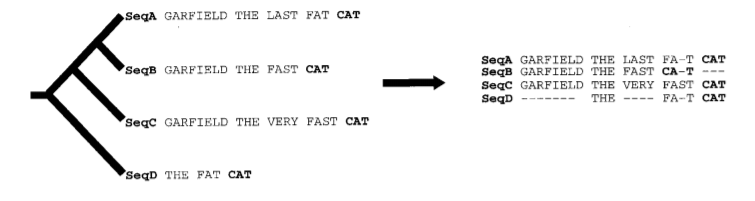
\includegraphics[scale=0.85]{t-coffee-errors}
\caption{Misalignment of the word CAT using other progressive methods. \citep[Figure~2(a)]{t_coffee}}
\end{figure}

Another method is MAFFT (the name presumably coming from the acronyms for multiple alignment and fast Fourier transform) \citep{mafft}.
The authors focused on finding alignments that are not only optimal, but also biologically correct. They developed a way of rapid identification
of homologous regions between two sequences using FFT, and then used the better pairwise alignments to create a better multiple alignment.

\subsubsection{T-Coffee}

The T-Coffee algorithm consists of various stages. The first one is to compute pairwise alignments for all pairs of input sequences.
Two primary libraries are generated, one for global and one for local alignments. Each can contain more than one alignment for each pair.

As some alignments tend to be more correct than others, weighting is then performed. The authors chose sequence identity of two aligned
sequences as the weight of each of the aligned residues in the pair. For example, consider the sequences $A$ \verb|GARFIELD THE LAST FAT CAT|
and $B$ \verb|GARFIELD THE FAST CAT|. If they are aligned as

\begin{verbatim}
    GARFIELD THE LAST FAT CAT
    GARFIELD THE FAST CAT ---
\end{verbatim}

then their sequence identity is 88\%, as there are two non-equal characters aligned (i.e. there is no gap penalty). Therefore, the weight of
each residue pair $W(A(x), B(y))$, where $A(x)$ denotes the character $x$ from sequence $A$, and analogically for $B(y)$, is equal to 88.

\begin{figure}[h]
\centering
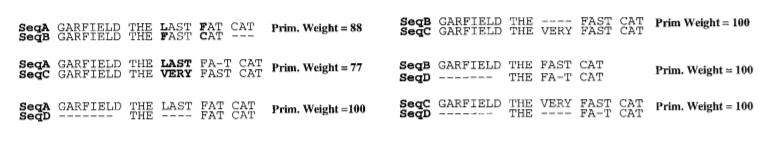
\includegraphics[scale=0.85]{t-coffee-primary-lib}
\caption{Primary library created from 4 sequences. \citep[Figure~2(b)]{t_coffee}}
\end{figure}

The two primary libraries are then combined into one by combining all identical residue pairs into one entry and summing their weights, while
pairs that are only present once are added with their original weight. Residue pairs that are not present in any alignment have an implicit weight
of 0.

Although the information present in the primary library is sufficient to obtain a multiple alignment, it is computationally hard to do so. Instead,
the authors chose to generate what they call an extended library using the weights in the primary library.

Library extension is performed by comparing each aligned residue pair with all the others. Consider a residue pair $(A(x), B(y))$ and a sequence $C$.
The initial weight of the pair is then increased by $min(W(A(x), C(z)), W(C(z), B(y)))$, i.e. the minimum weight associated to the alignment of some
residue $C(z)$ with both $A(x)$ and $B(y)$. This is done for all residues from all sequences. In practice, most of the weights will be 0, therefore 
the actual algorithm computes the weights more efficiently. Library extension in effect computes how consistent a residue-pair alignment is.

\begin{figure}[h]
\centering
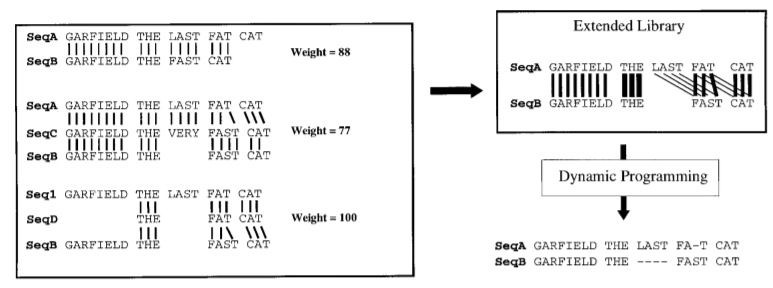
\includegraphics[scale=0.85]{t-coffee-extended-lib}
\caption{Extended library weights for two sequences and their alignment recomputed using these weights. \citep[Figure~2(c)]{t_coffee}}
\end{figure}

Having obtained the consistency information from the extended library, it is now possible to create the guide tree and the final multiple alignment.
Using a distance matrix between all the sequences, the tree is computed as follows. First, we align the closest two sequences using dynamic programming
and the weights from the extended library. In each of the following steps, we either add a sequence to an already computed alignment, or we align
the next closest sequences. We repeat this step until the alignment of all sequences is complete.

\begin{figure}[h]
\centering
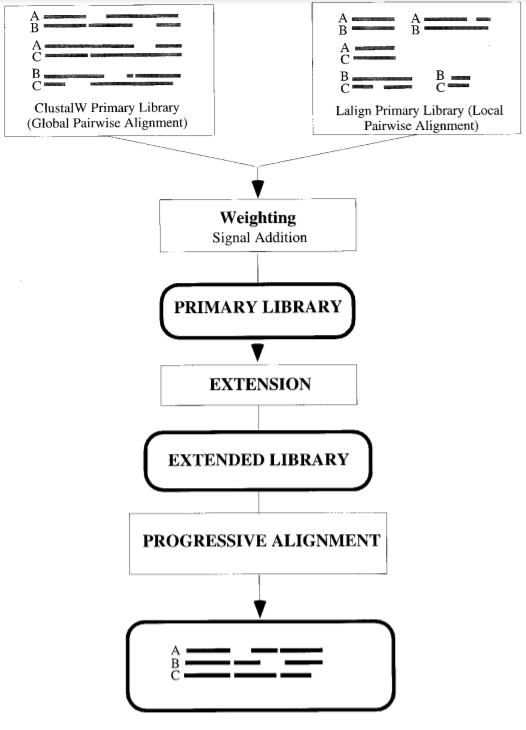
\includegraphics[scale=0.5]{t-coffee-flowchart}
\caption{T-Coffee layout. \citep[Figure~1]{t_coffee}}
\end{figure}

\subsubsection{MAFFT}

The MAFFT method is similar to T-Coffee in that it constructs a library of alignments which it then uses to create the final multiple alignment. The authors developed MAFFT
to work in multiple modes, one of which is the progressive method as described above; the other one is the iterative refinement method, which allows for alterations
of the multiple alignment obtained from the progressive method.

Pairwise alignment in MAFFT uses the fact that certain amino acids have more similar physico-chemical properties than others. Substitutions tend to preserve the
overall structrure of a protein, therefore substitutions of similar amino acids are more frequent than those of different ones. The two properties
the authors use are amino acid volume and polarity.

Let us define the correlation of the volume component between two amino acid sequences with the positional lag of $k$ as

\[
    c_v(k) = \sum_{1\leq n \leq N, 1 \leq n+k \leq M} \hat{v}_1(n) \hat{v}_2(n+k)
\]
where $N$ and $M$ are the lengths of the sequences and $\hat{v}(a) = [v(a) - \bar{v}] / \sigma_v$ is the normalized volume value with $\bar{v}$
denoting the average volume of all the amino acids and $\sigma_v$ their standard deviation.

Since the sequences tend to be equal in length, computing $c_v(k)$ using naive methods takes time proportional to $N^2$. However, applying Fast Fourier
transform to the calculation reduces the time to $\mathcal{O}(N log N)$.

We define the polarity component correlation $c_p(k)$ analogically.

The correlation between two amino acids is then expressed as 

\[
    c(k) = c_v(k) + c_p(k)
\]

\begin{figure}[h]
\centering
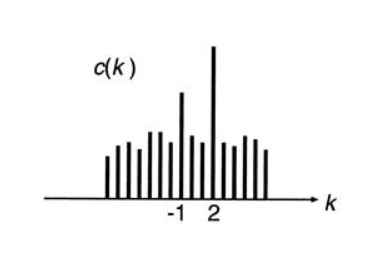
\includegraphics{mafft_correlation_plot}
\caption{Plot of the correlation function $c(k)$. \citep[Figure~1A]{mafft}}
\label{fig:mafft1}
\end{figure}

If we plot the function $c(k)$, there will be some peaks corresponding to the homologous regions of the two sequences, if there are any (Figure \ref{fig:mafft1}). However, the FFT
analysis only gives us the positional lag of the regions, not their positions. To find the exact positions, we use a sliding window (of size 30 in the article)
and calculate the degree of local homologies for the 20 highest peaks in the $c(k)$ function. If a segment exceeding a given homology threshold is identified,
we label it as a homologous region.

\begin{figure}[h]
\centering
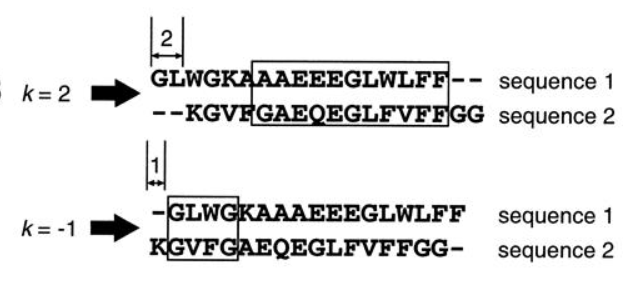
\includegraphics{mafft_sliding_window}
\caption{Finding homologous regions with different positional lags using a sliding window. \citep[Figure~1B]{mafft}}
\label{fig:mafft2}
\end{figure}

After finding homologous segments between two sequences, their alignment is obtained by constructing a homology matrix $S \in R^{n*n}$, where $n$ is the number of homologous
segments. The cell $S_{ij}$ is assigned a value depending on whether the $i$-th homologous segments of the first sequence corresponds to the $j$-th homologous segment
of the second sequence. If so, the cell gets a value corresponding to the score of this segment; otherwise it has a value of 0. The optimal arrangment of homologous segments
is then obtained using dynamic programming.

\begin{figure}[h]
\centering
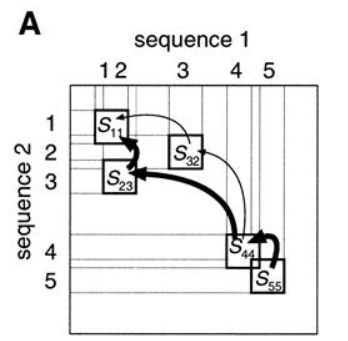
\includegraphics{mafft_optimal_path}
\caption{Dynamic programming applied on segment arrangement. \citep[Figure~2A]{mafft}}
\label{fig:mafft3}
\end{figure}

Having arranged homologous segments, the algorithm then computes pairwise alignments for each pair of sequences. As in T-Coffee, it uses the alignments to create
the primary and extended libraries, which are in turn used to estimate the guide tree and the final alignment. If MAFFT is configured to perform the progressive 
method, this alignment is the final one. Otherwise, if iterative refinement is allowed, MAFFT uses the weights from the library to adjust the alignment to get a more
optimal one. However, iterative refinement is very slow from a relatively low number of sequences, therefore it is not suitable for a large dataset.

\section{Sequence alignment for chant melodies}

As we have discussed before, melodies of Gregorian chant are in many ways similar to biological sequences. The alphabet is different (instead of 20 amino acids
in proteins or 4 nucleotide bases in DNA we have around 40 different characters used in melody representation) and the chants are usually shorter in length.
The evolution of both biological and melodic sequences is guided by environmental factors such as migration to other places. Some segments tend to undergo a lot
of modifications, while other remain relatively unchanged. Studying the alignment of chant melodies can reveal a lot of information about their relationship.

In the following sections, we describe three approaches to melody alignment used in our application.

The first one is a naive approach. It merely aligns all chants to have the same number of words and each word to have the same number of syllables, filling the extra
positions with gaps, if needed.

The other two approaches use MAFFT to perform a proper sequence alignment. They differ in what we are aligning. One of them aligns notes and other symbols as they are;
each representing a certain pitch. The other one is more sophisticated: it does not use the absolute value of the pitches, but rather the intervals between the notes.
This way, we can see segments that have merely been shifted by a certain interval.

\subsection{Naive alignment}

\subsection{Multiple alignment using absolute pitches}

For this task, we are using the MAFFT software\footnote{https://mafft.cbrc.jp/alignment/software/}. As the software uses the character \verb|-| for marking gaps,
it requires that the input sequences do not contain any, or they will be removed. Since melodies encoded as Volpiano use the character to mark ends of words
and ends of syllables, we need to perform some preprocessing. Namely, we replace all contiguous sequences \verb|---| with the end-of-word marking symbol \verb|~|
and all contiguous sequences \verb|--| with the end-of-syllable marker \verb=|=. All remaining \verb|-|s are removed, if there are any.

The sequences are then passed to MAFFT with the option \verb|--text|, which indicates that the sequences are not biological. Additionally, we also pass the option
\verb|--reorder|, which returns the aligned sequences in order of similarity. We made this choice so as to facilitate the identification of related melodies.

After MAFFT performs the alignment, we retrieve the sequences and attempt to combine them with their text.
We do this by splitting both the text and the melody into syllables and mapping them onto each other (Algorithm \ref{algo:volpiano_text_combine}). 
However, this might not be possible. Due to errors in the original encoded melody (i.e. a missing or an extra \verb|-|),
we may have altered the structure of the chant in preprocessing. In case of such event, we remove the affected sequence from consideration and align the remaining
sequences again.\newline

\begin{algorithm}[H]
\SetKwInOut{Input}{input}\SetKwInOut{Output}{output}
    \Input{\emph{volpiano}: melody divided into words and those into syllables, and \emph{text}: lyric divided analogically}
    \Output{\emph{volpiano} and \emph{text} aligned}
    \BlankLine
    set \emph{aligned\_text\_and\_melody} to be an empty list\;
    \For{word at index i}{
        open new word in \emph{aligned\_text\_and\_melody}\;
        \uIf{i-th word of text has more syllables than i-th word of melody}{
            merge the extra syllables into the last one\;
        }
        \uElseIf{i-th word of text has fewer syllables than i-th word of melody}{
            extend the i-th word of text by empty syllables to match the volpiano word
        }
        \For{syllable at index j of i-th word}{
            combine text and melody of the j-th syllable of the i-th word and add it to the current word\;
        }
        close current word\;
    }
    return \emph{aligned\_text\_and\_melody}\;
    \caption{Aligning melody and lyric}
    \label{algo:volpiano_text_combine}
\end{algorithm}

Once all sequences are successfully aligned without errors in text and melody combination, we can display them to the user. In the application, we use the Volpiano font,
so as to maintain consistency. However, the sequences shown are not properly encoded in Volpiano format. First of all, we choose different representations of end of a word
(here we use a bar line) and end of a syllable (a single space) so that the number of characters in each sequence remains equal and the alignment is visible. Second of all,
after the alignment, MAFFT will have inserted \verb|-|s to represent gaps. In proper Volpiano, these characters represent gaps between words, syllables, and neumes. However,
here they just mean empty space.\newline

\begin{algorithm}[H]
\SetKwInOut{Input}{input}\SetKwInOut{Output}{output}
    \Input{a set of volpiano-encoded melodies with their respective lyrics}
    \Output{aligned melodies combined with their lyrics}
    \BlankLine
    preprocess all melodies to a MAFFT-friendly format\;
    \While{melodies have not been aligned without error}{
        run MAFFT on all melodies\;
        \For{aligned melody}{
            combine melody with its text\;
            \If{melody and text cannot be combined}{
                remove melody from list\;
                remember to run the while loop again\;
            } 
        }
    }
    return list of aligned melodies combined with their texts\;
    \caption{Multiple alignment using absolute pitches}
    \label{algo:align_pitch}
\end{algorithm}

\subsection{Multiple alignment using intervals}

The general outline of the algorithm is the same as Algorithm \ref{algo:align_pitch}. However, as we are not aligning absolute pitches, but rather intervals,
we need to compute these intervals.

There are 18 possible pitches, which means 37 possible intervals (17 positive, 17 negative, and one without the change of pitch). We will represent the no-change interval
with the character \verb|a|, the positive intervals with the lowercase characters \verb|b-t| and the negative intervals with the uppercase characters \verb|B-T|. The characters
\verb|i| and \verb|I| are not used for reasons explained later.

The interval representation is constructed from a Volpiano-encoded melody by replacing the note symbols with the appropriate interval symbol. The $i$-th note will be
replaced with the symbol representing the interval $(i-1, i)$. As the first note has no predecessor, it is left as it is. The non-note symbols also remain unchanged.\newline

\begin{algorithm}[H]
\SetKwInOut{Input}{input}\SetKwInOut{Output}{output}
    \Input{volpiano-encoded melody}
    \Output{interval representation of the input melody}
    \BlankLine
    $interval\_representation \longleftarrow ""$\;
    \For{character c in volpiano}{
        \uIf{c is a non-note character}{
            append c to \emph{interval\_representation}\;
        }
        \uElseIf{c is a note-representing character and it is the first such one}{
            append c to \emph{interval\_representation}\;
            $last\_seen\_note \longleftarrow c$\;
        }
        \uElse{
            $interval \longleftarrow (last\_seen\_note, c)$\;
            $i \longleftarrow symbol \: for \: interval$\;
            append i to \emph{interval\_representation}\;
            $last\_seen\_note \longleftarrow c$\;
        }
    }
    return \emph{interval\_representation}\;
    \caption{Converting volpiano-encoded melody into interval representation}
    \label{algo:convert_to_interval}
\end{algorithm}

We use the interval representations as inputs to MAFFT. That means that what MAFFT returns are the aligned sequences of intervals. To display them to the user
properly, we need to decode the sequences.\newline

\begin{algorithm}[H]
\SetKwInOut{Input}{input}\SetKwInOut{Output}{output}
    \Output{interval representation of a melody}
    \Input{volpiano-encoded equivalent of the input melody}
    \BlankLine
    $volpiano \longleftarrow ""$\;
    \For{character c in interval representation}{
        \uIf{c is a non-interval character}{
            append c to \emph{volpiano}\;
        }
        \uElseIf{c is a note-representing character and it is the first such one}{
            append c to \emph{volpiano}\;
            $last\_seen\_note \longleftarrow c$\;
        }
        \uElseIf{c is an interval-representing character and we have already seen the first note}{
            $note \longleftarrow last\_seen\_note +$ interval represented by $i$\;
            append note to \emph{volpiano}\;
            $last\_seen\_note \longleftarrow note$\;
        }
    }
    return \emph{volpiano}\;
    \caption{Converting interval representation back to volpiano}
    \label{algo:decode_interval}
\end{algorithm}

The reason why we are not using \verb|i| and \verb|I| as symbols for an interval is that as we are looking at whether a character is a note or an interval or neither, 
if they represented an interval, we would choose the appropriate branch in Algorithm \ref{algo:decode_interval}. However, marking an interval is not the only way how
the character could have got there: \verb|i| and \verb|I| represent non-note elements in the Volpiano protocol. Therefore, we could mistakenly shift the melody by an interval,
as there is no way of knowing which case it is.

The complete algorithm is similar to Algorithm \ref{algo:align_pitch}.\newline

\begin{algorithm}[H]
\SetKwInOut{Input}{input}\SetKwInOut{Output}{output}
    \Input{a set of volpiano-encoded melodies with their respective lyrics}
    \Output{aligned melodies combined with their lyrics}
    \BlankLine
    convert all melodies to interval representations\;
    preprocess all interval representations to a MAFFT-friendly format\;
    \While{melodies have not been aligned without error}{
        run MAFFT on all interval representations\;
        \For{aligned interval representation}{
            convert interval representation to volpiano-encoded melody\;
            combine melody with its text\;
            \If{melody and text cannot be combined}{
                remove melody from list\;
                remember to run the while loop again\;
            } 
        }
    }
    return list of aligned melodies combined with their texts\;
    \caption{Multiple alignment using intervals}
    \label{algo:align_intervals}
\end{algorithm}

\chapter{User documentation}

This application is a tool for analyzing user-defined data. It comes with some data already provided, however, it does not substitute the
function of database webs.

The application is a locally-run web application. It can be accessed via a web browser by navigating to the corresponding URL.\footnote{
In the default settings, this URL is \url{localhost:4200}.} Setup instructions can be found in attachment \ref{attachment:setup}.

In this chapter, we present an overview of the functionality of the application. The first section sketches out the overall
functionality of the application. The following sections describe each feature in more detail.


\section{Site map}

Figure \ref{fig:sitemap} shows a sitemap of the application. It shows how the site can be navigated to get to the different functions.
The rectangles represent pages with their own URLs, while the ellipses represent the pages' functions.

\begin{figure}[!h]
\centering
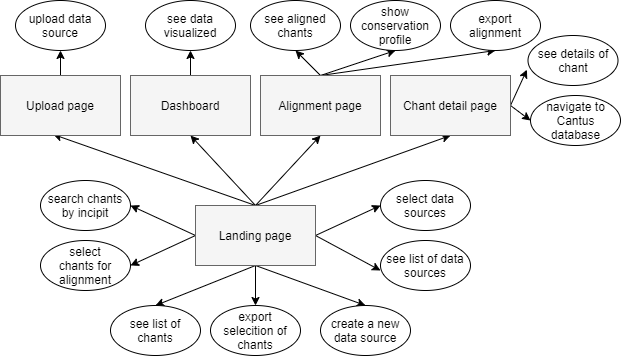
\includegraphics[scale=0.65]{udocs_sitemap}
\caption{Sitemap of the application.}
\label{fig:sitemap}
\end{figure}

\section{Landing page}

The application contains one or more data sources. A data source is a set of chant data defined by the user. The application comes with one data
source, \emph{CantusCorpus v0.2}, already uploaded. The separation of data sources enables users to compare different datasets.

The landing page provides several functions (see Figure \ref{fig:land_page}). The top panel, which is always present on the page, allows for quick
navigation to other pages and for filtering search by chants' incipit (the first few words of text). It shows a list of chants from the current search
settings, as well as a filter panel used for modifying the settings. There is an option to export a selection of chants to a CSV file and to create a new
data source from them, as well as several options for their alignment.

The panel on the right side enables data source selection. To change data source (more than one can be selected at once), click the checkbox next
to the data source name and click \emph{save}. To hide or unhide the data source panel, click on the black \emph{Data sources} button. The panel
is available in the entire application.

\begin{figure}[!h]
\centering
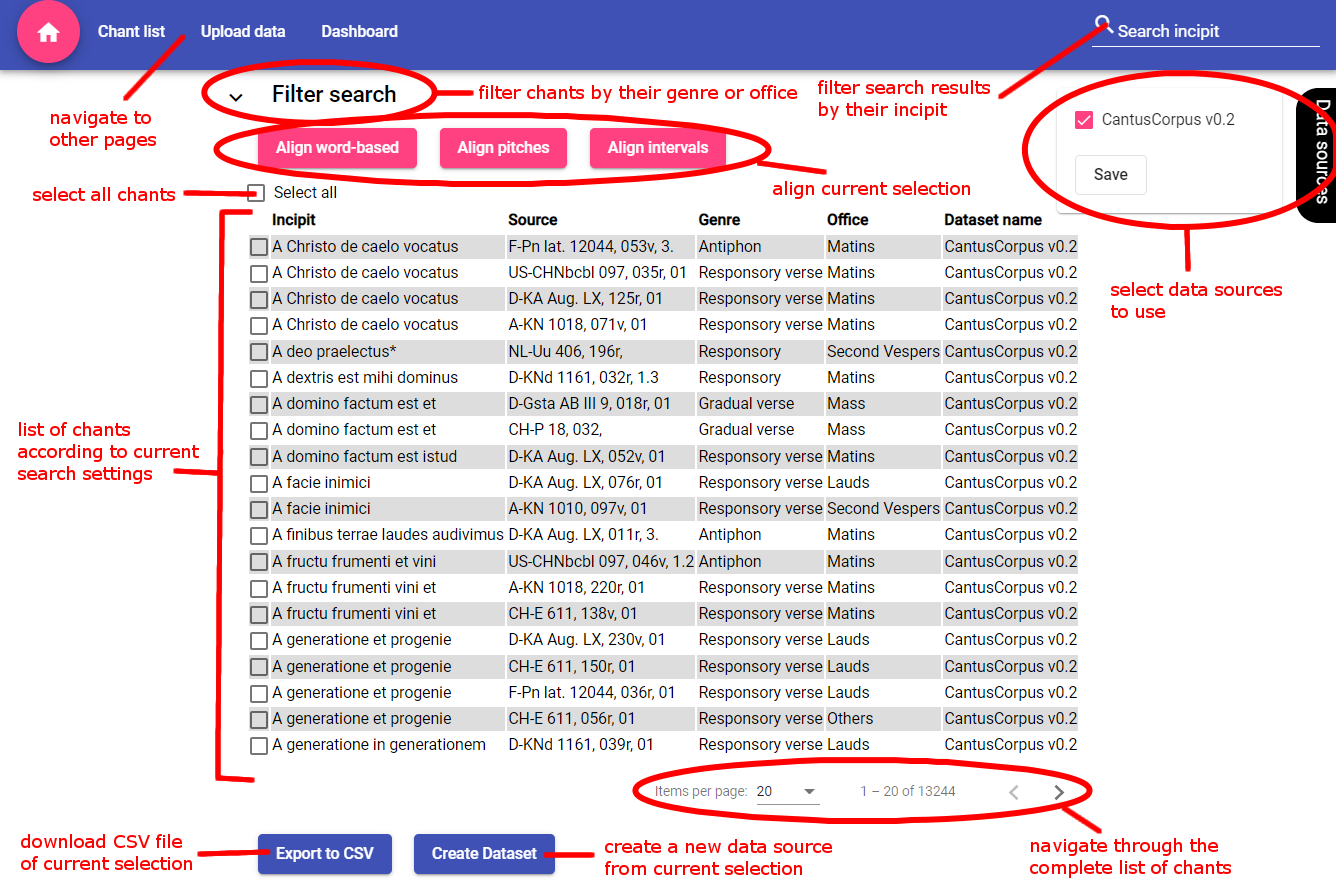
\includegraphics[scale=0.5]{udocs-homepage-marked}
\caption{Landing page and its features.}
\label{fig:land_page}
\end{figure}

\subsection{List of available chants}

The landing page displays a list of chants from a specified source, which is by default set to the provided data source \emph{CantusCorpus v0.2}.
As we assume that the number of all selected chants can be large, we do not display all of them at once. Instead, the user can choose the number of
chants displayed at once and paginate through the list to get to later ones.

Some elements of the list have an incipit ending with an asterisk (\verb|*|). This indicates that the specific chant does not have its entire
text transcribed, only the part in the incipit.

\subsection{Incipit search}

The landing page provides the possibility to filter chants from the current selection by their incipit (the first few words of the chant). To do so, enter the desired string into
the field in the top-right corner marked as \emph{Search incipit} and press Enter (Figure \ref{fig:inc-search}). A set of chants that contain the query as
a substring (not necessarily as a prefix) of their incipit will be displayed (Figure \ref{fig:inc-search-result}). Be aware that a misspelled query will not return the correct results.

\begin{figure}[!h]
\centering

\includegraphics{udocs-search-incipit}
\caption{Entering search query into the \emph{Search incipit} box.}
\label{fig:inc-search}
\end{figure}

\begin{figure}[!h]
\centering
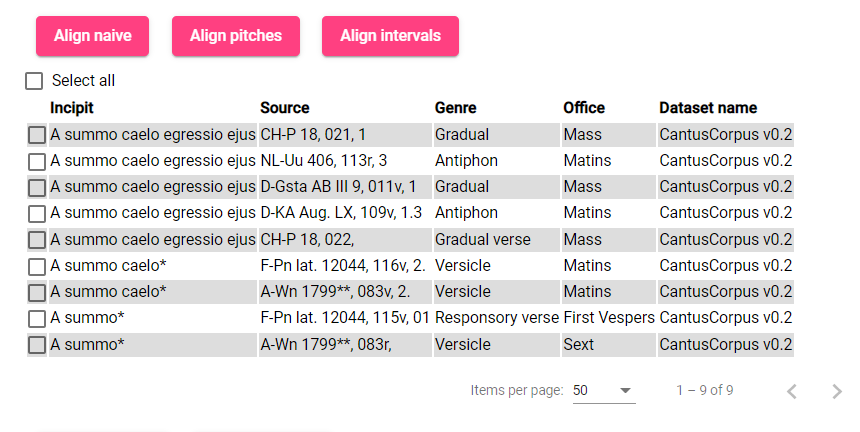
\includegraphics[scale=0.6]{udocs-after-incipit-search}
\caption{The result of the query. Notice that each incipit has the query as a substring.}
\label{fig:inc-search-result}
\end{figure}

\subsection{Search filter}

It is possible to filter the search results by their genre and office. The filter panel can be opened by clicking the down arrow next to the \emph{Filter search}
heading. By default, all genres and all offices are selected. To select or unselect some of them, click the checkbox next to their abbreviation. To select 
or unselect all genres or offices, click the checkbox next to \emph{All} in the respective section (Figure \ref{fig:search_filter}).

The filter panel does not use the full names of the genres and offices, as in some cases, the name can be very long. Instead, it uses their abbreviations as used 
in Cantus Index. Attachments \ref{attachment:genres} and \ref{attachment:offices} provide a list of genres, resp. offices and their abbreviations.

\begin{figure}[!h]
\centering
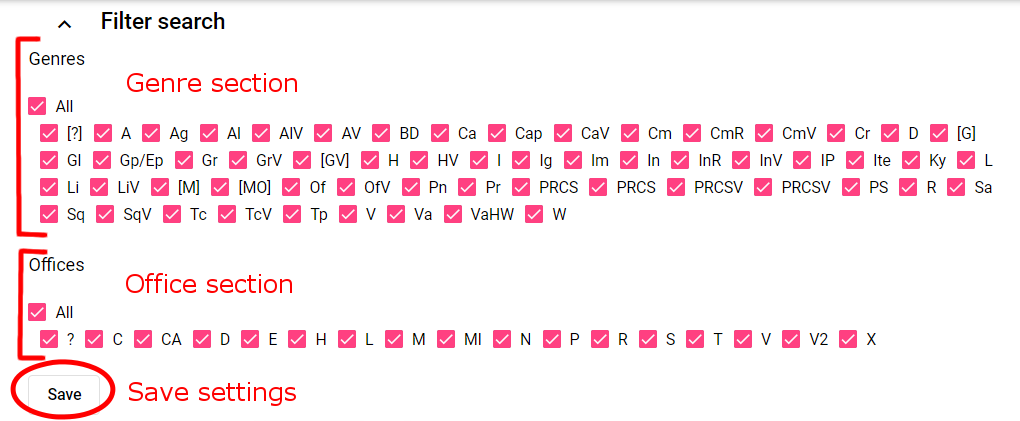
\includegraphics[scale=0.5]{udocs-filter-marked}
\caption{Search filter panel.}
\label{fig:search_filter}
\end{figure}

\subsection{Chant detail}

By clicking on a chant's incipit in the search results list, the user is redirected to a page which displays the chant's melody with the text in full,
as well as other information of interest. It shows the chant's Cantus ID, by which it can be found in the Cantus Database. It also shows a URL which
points to the corresponding entry on the Cantus website (Figure \ref{fig:chant-detail}). These fields are valid for all chants from the default
\emph{CantusCorpus v0.2} dataset, but there is no guarantee of their correctness in user-uploaded data.

\begin{figure}[!h]
\centering
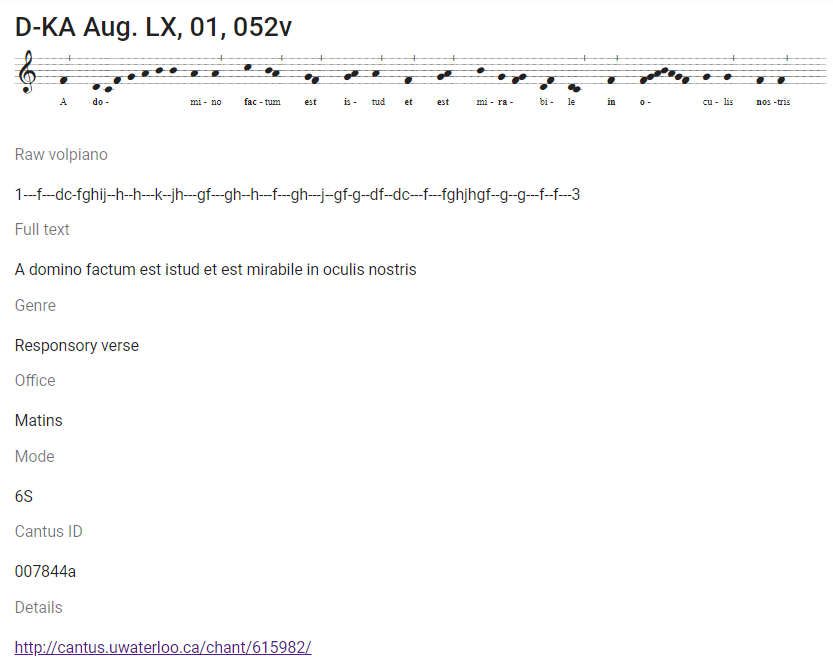
\includegraphics[scale=0.6]{udocs-chant-detail}
\caption{Page with the detail of the selected chant.}
\label{fig:chant-detail}
\end{figure}

\subsection{Data export}
\label{section:data_export}

The user may wish to export the results of their search into a CSV file. In that case, select the desired chants by checking the checkbox next to
their incipit (or \emph{Select all}) and click the \emph{Export to CSV} button at the bottom of the page. A file with the name \emph{dataset.csv}
will be automatically downloaded (Figure \ref{fig:export-ex}).

\begin{figure}[!h]
\centering
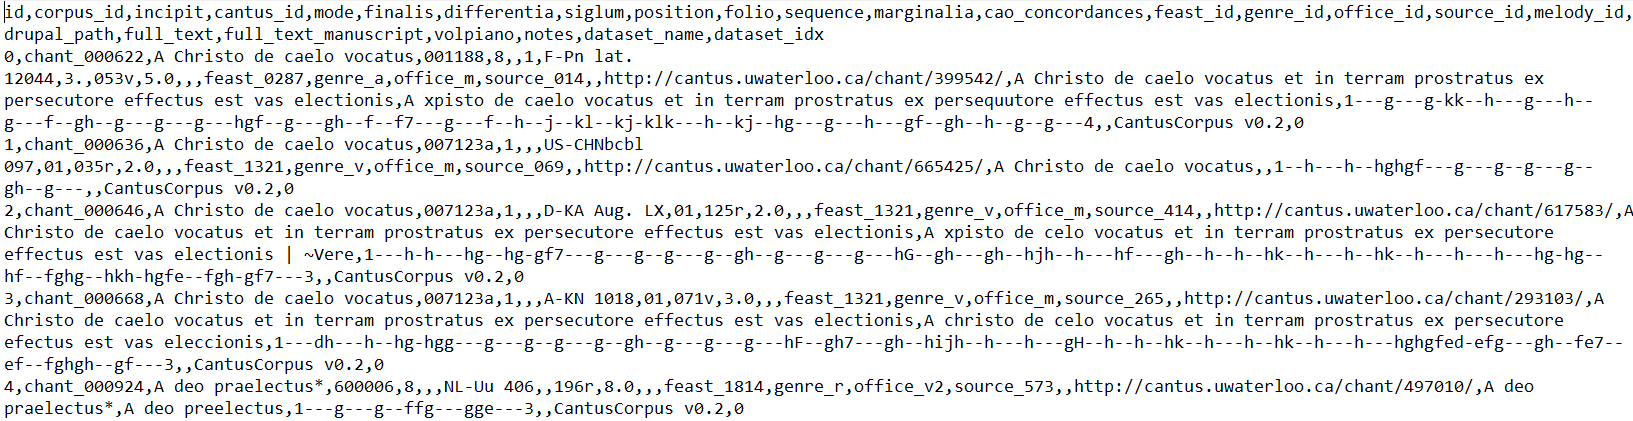
\includegraphics[scale=0.4]{udocs-exported-ds}
\caption{First few lines of the exported CSV file.}
\label{fig:export-ex}
\end{figure}

\section{Data source creation}

The application is not limited to the data present by default. The user can either create a data source from their search results, or upload
completely new data.

\subsection{Create from search}

To create a data source from the search results, check the checkboxes next to the desired chants and click the \emph{Create Dataset} button at the bottom
of the page. The user will be prompted for the data source name (Figure \ref{fig:create-ds}). If no name is entered, the name of the data source will be
\emph{undefined}. After confirming the name, the data source list will be automatically updated with the newly-created one (Figure \ref{fig:update-ds-antiphons}).

\begin{figure}[!h]
\centering
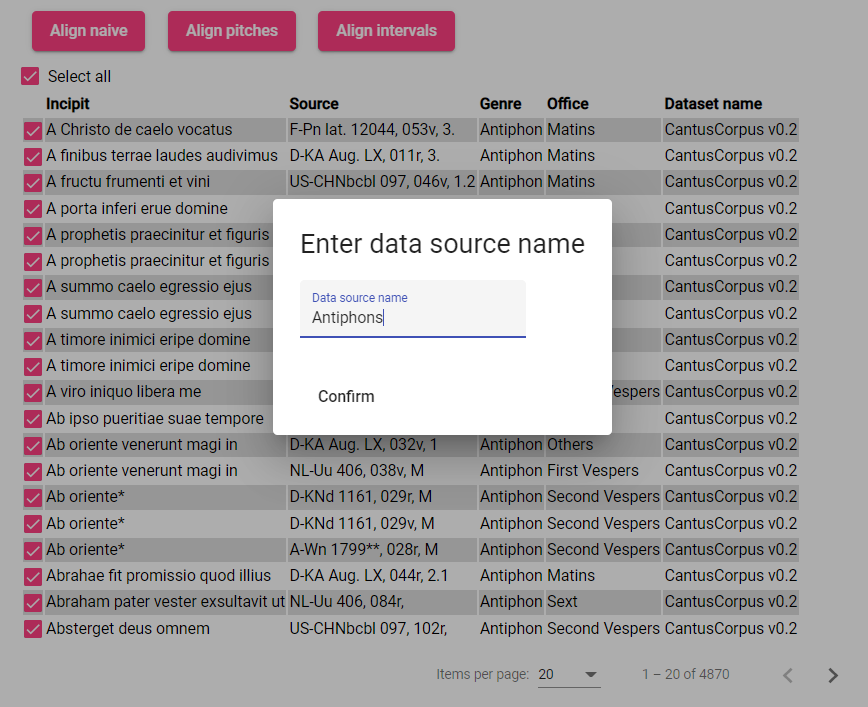
\includegraphics[scale=0.6]{udocs-create-ds}
\caption{Prompt for entering the name of the data source appears after clicking the \emph{Create Dataset} button.}
\label{fig:create-ds}
\end{figure}

\begin{figure}[!h]
\centering
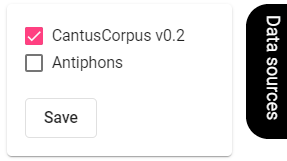
\includegraphics{udocs-ds-in-list}
\caption{The newly created data source automatically appears in the data source list.}
\label{fig:update-ds-antiphons}
\end{figure}

\subsection{User data upload}

To upload new data, navigate to the \emph{Upload data} page in the top panel. Select the file to upload and enter the data source name (Figure \ref{fig:upload-ds}). The file should be
in CSV format and its contents are specified in Section \ref{section:data_usr}. Click \emph{Upload} to upload the file. After the file is processed, the data source list will
be automatically updated (Figure \ref{fig:update-ds-respon}). The exported file created in Section \ref{section:data_export} is suitable for upload.

\begin{figure}[!h]
\centering
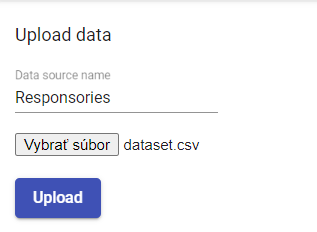
\includegraphics{udocs-upload-respon}
\caption{The upload form with the file \emph{dataset.csv} selected for upload. The new data source will have the name \emph{Responsories}.}
\label{fig:upload-ds}
\end{figure}

\begin{figure}[!h]
\centering
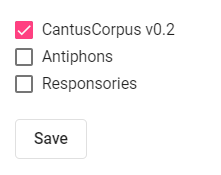
\includegraphics{udocs-ds-with-respon}
\caption{The uploaded data source automatically appears in the list.}
\label{fig:update-ds-respon}
\end{figure}

\section{Alignment}

The alignment tool is the core functionality of the application.

It is possible to select a set of chants and have them be aligned using one of the methods described in Section \ref{section:chant_alignment}. The alignment option is selected by clicking
on one of the buttons above the chant list (see Figure \ref{fig:land_page}) after selecting the chants to be aligned. After doing so, the user is redirected to a page where the alignment result
is shown. In some cases, the alignment make take up to a minute to complete.

The alignment result is shown as a list of melodies (Figure \ref{fig:align-result}). The melodies are either arranged in the same order as they were displayed in the chant list (in the case of
naive alignment) or in the order of similarity.

\begin{figure}[!h]
\centering
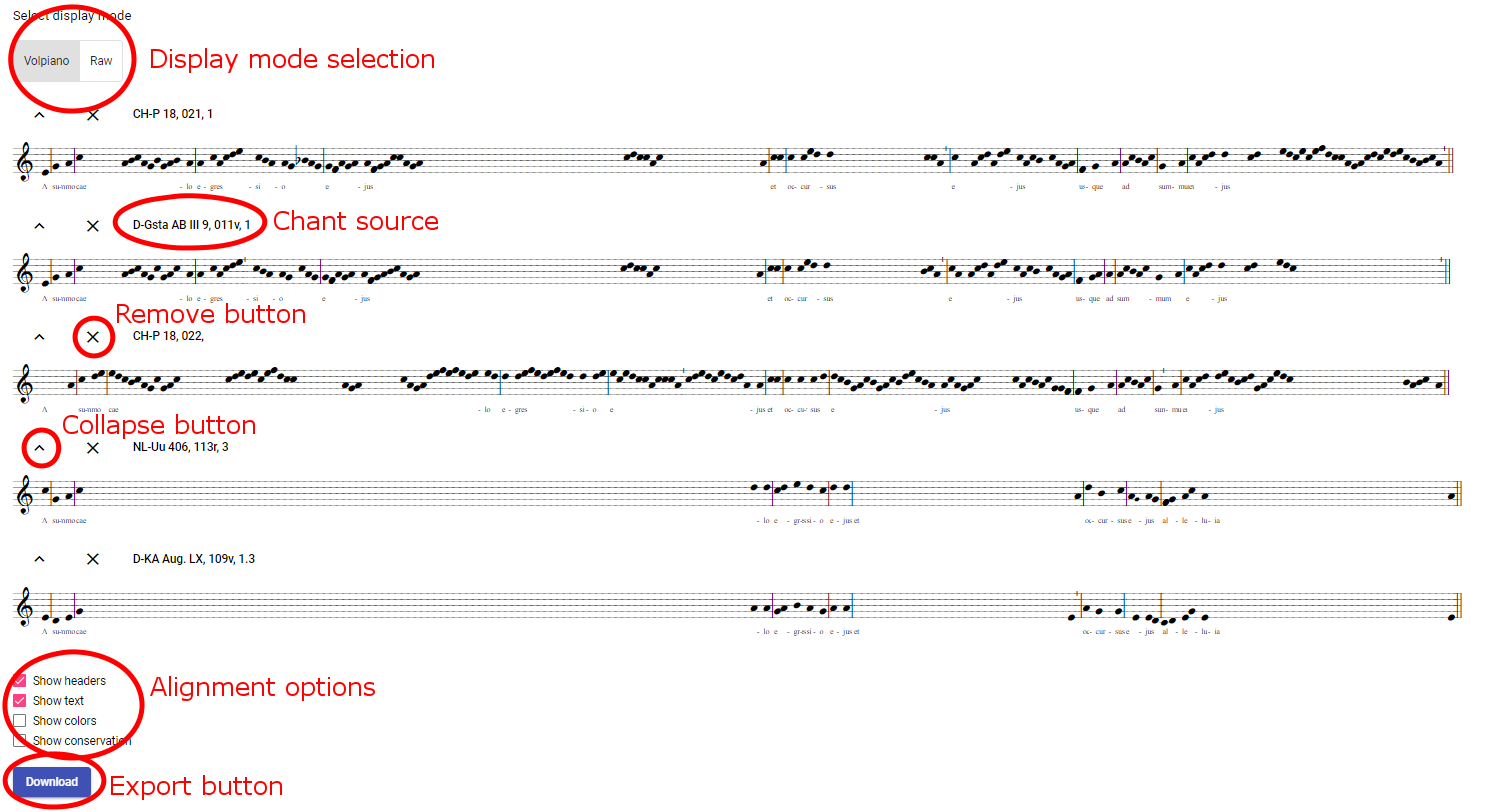
\includegraphics[scale=0.4]{udocs-alignment-basic-marked}
\caption{Result of the alignment.}
\label{fig:align-result}
\end{figure}

To show more information about each melody, the user can click on the chant source button by which each chant is identified. The same information as when navigating
to the chant's page is displayed (Figure \ref{fig:align-detail}). To hide the detail, click on the chant source button again.

\begin{figure}[!h]
\centering
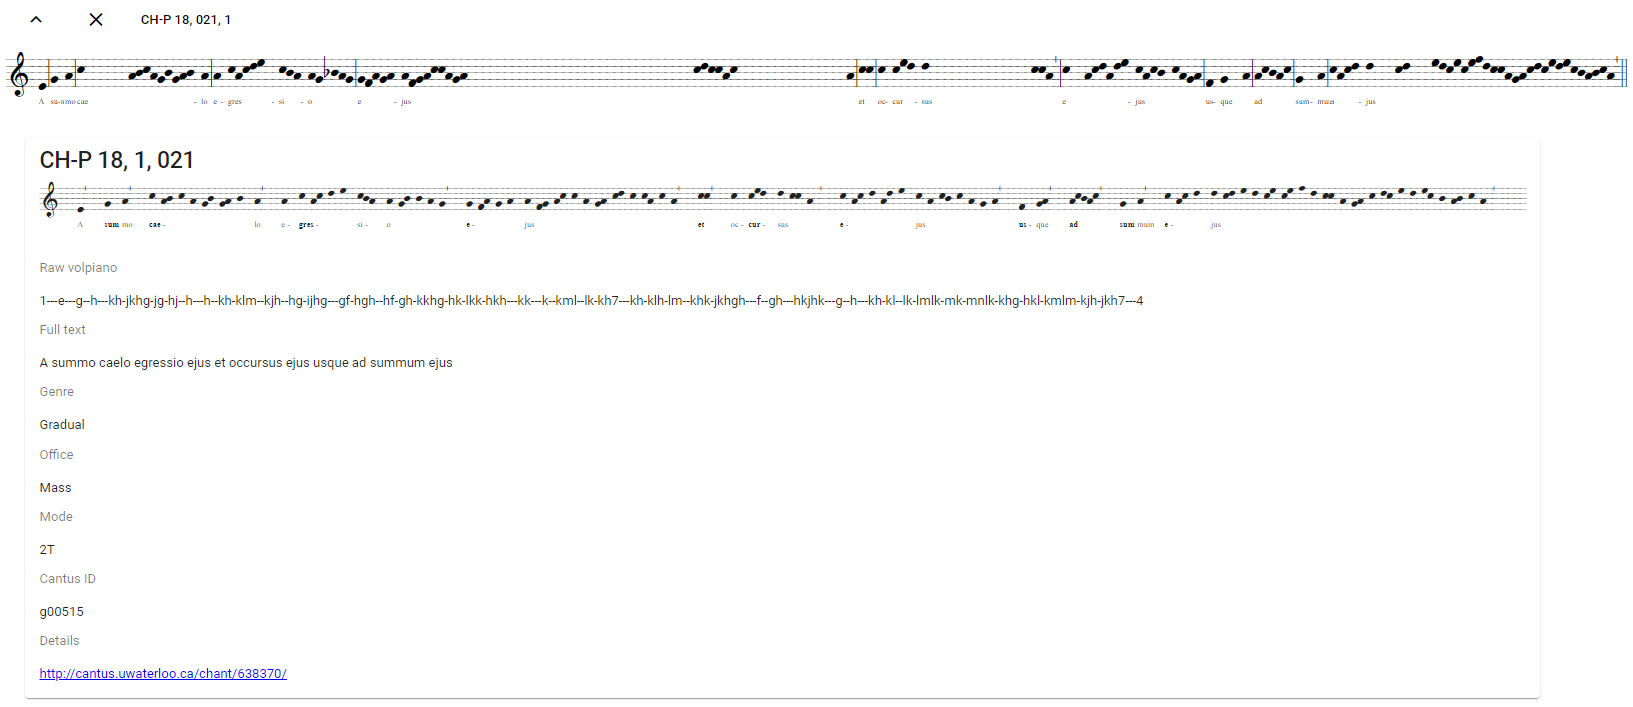
\includegraphics[scale=0.4]{udocs-alignment-detail}
\caption{Aligned melody with the chant information displayed.}
\label{fig:align-detail}
\end{figure}

If the user wishes to rearrange the displayed melodies, simply click anywhere close to a melody and drag it to another position (Figure \ref{fig:align-rearrange}).

\begin{figure}[!h]
\centering
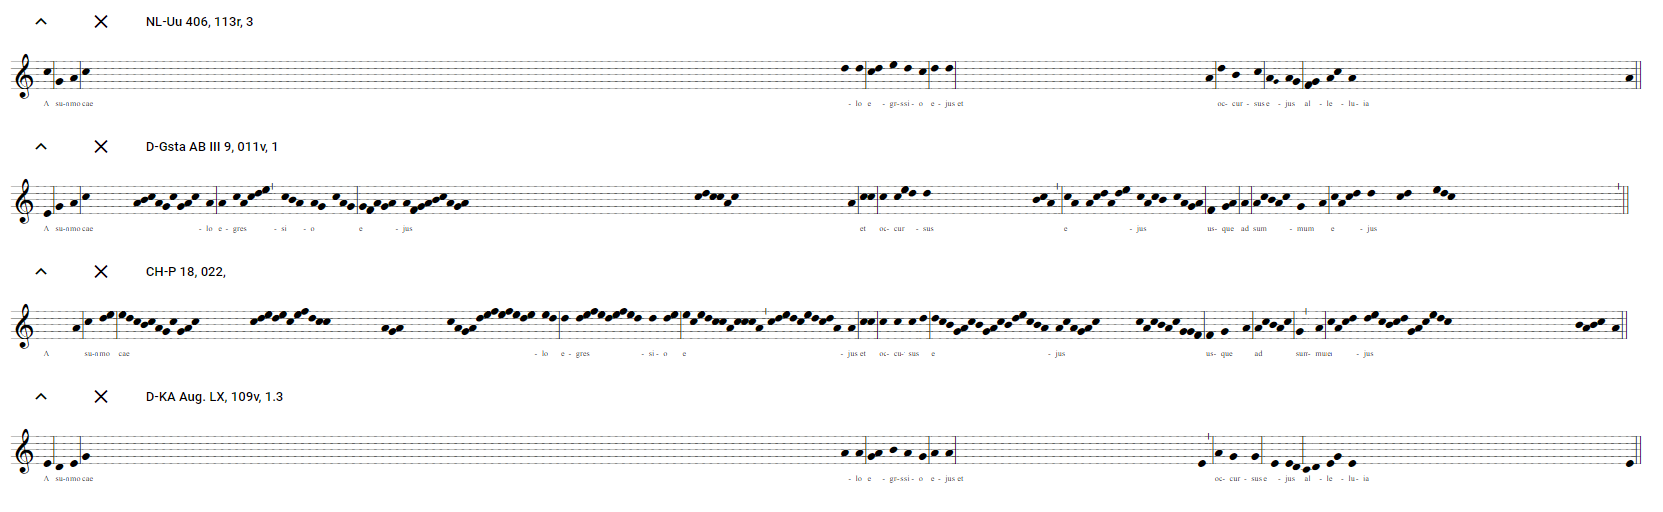
\includegraphics[scale=0.4]{udocs-alignment-rearrange}
\caption{Alignment after dragging and dropping the last melody. Compare to Figure \ref{fig:align-result}.}
\label{fig:align-rearrange}
\end{figure}

\subsection{Collapsing and deleting alignment}

After the alignment is shown, the user can choose to collapse the alignment (i.e. hide the notes) by clicking on the \emph{Collapse} button (Figure \ref{fig:align-collapsed})
in each melody's header or to remove it completely by clicking on the \emph{Remove button} (Figure \ref{fig:align-removed}). The chant can be uncollapsed by clicking
on the same button. However, removing the chant entirely is permanent. To get the removed chant back, the page needs to be reloaded.

\begin{figure}[!h]
\centering
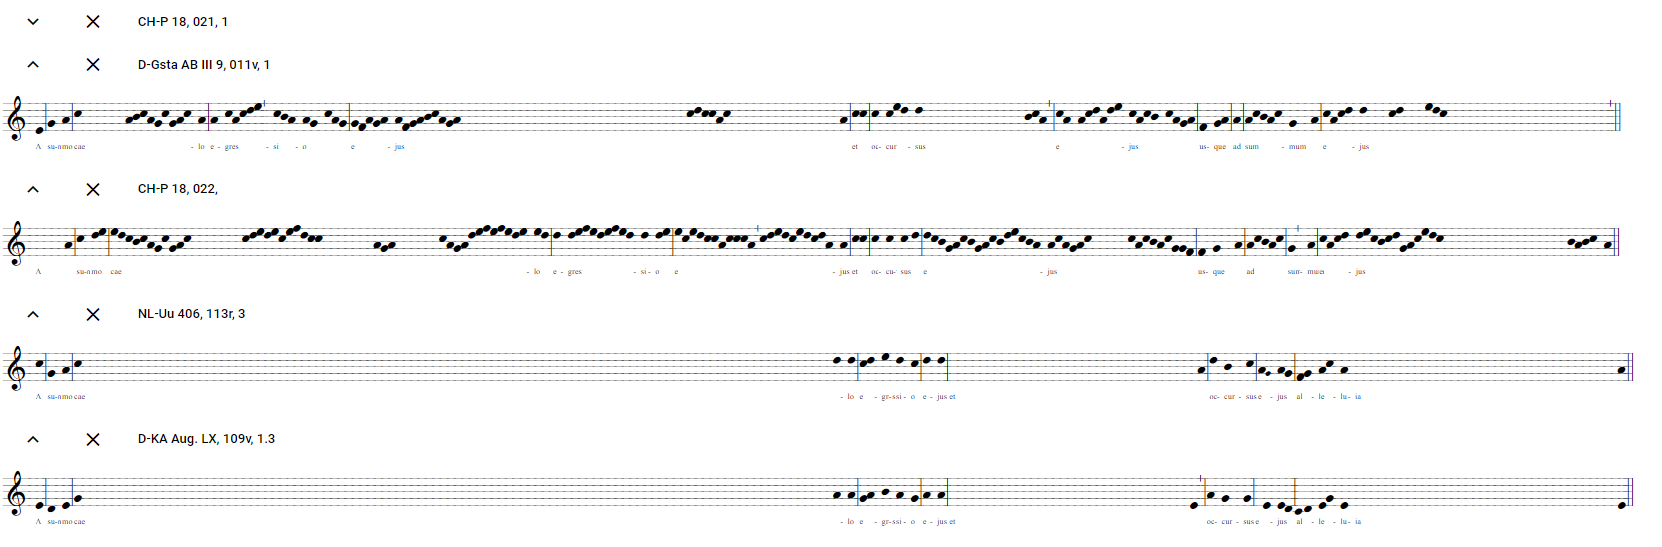
\includegraphics[scale=0.4]{udocs-alignment-collapsed}
\caption{The first chant is collapsed.}
\label{fig:align-collapsed}
\end{figure}

\begin{figure}[!h]
\centering
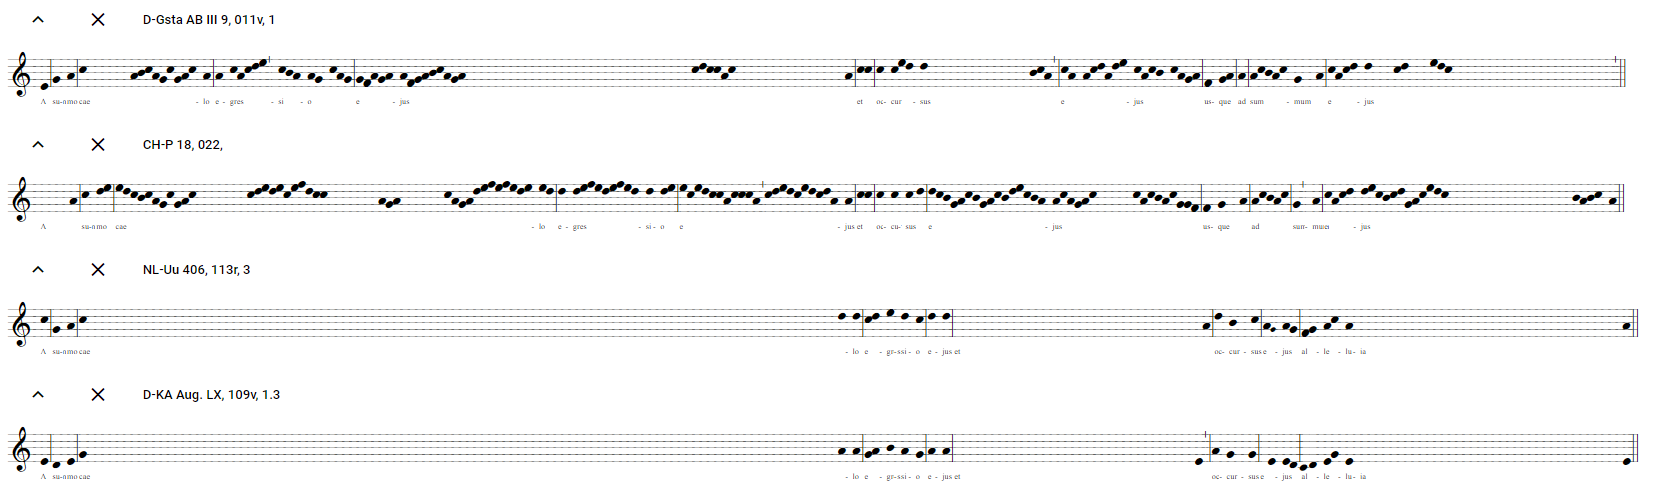
\includegraphics[scale=0.4]{udocs-alignment-deleted}
\caption{The first chant is removed. Compare to Figure \ref{fig:align-result}.}
\label{fig:align-removed}
\end{figure}

\subsection{Alignment display options}

Once the chants have been aligned, there exist several options to better show how they are aligned.

As the Volpiano font does not have characters of equal width, the notes that are actually aligned might not be shown as aligned. To see the
actual alignment, the user can change the display mode above the aligned melodies to \emph{Raw}, which shows the melodies as the encoded string
in a monopaced font (Figure \ref{fig:align-raw}).

\begin{figure}[!h]
\centering
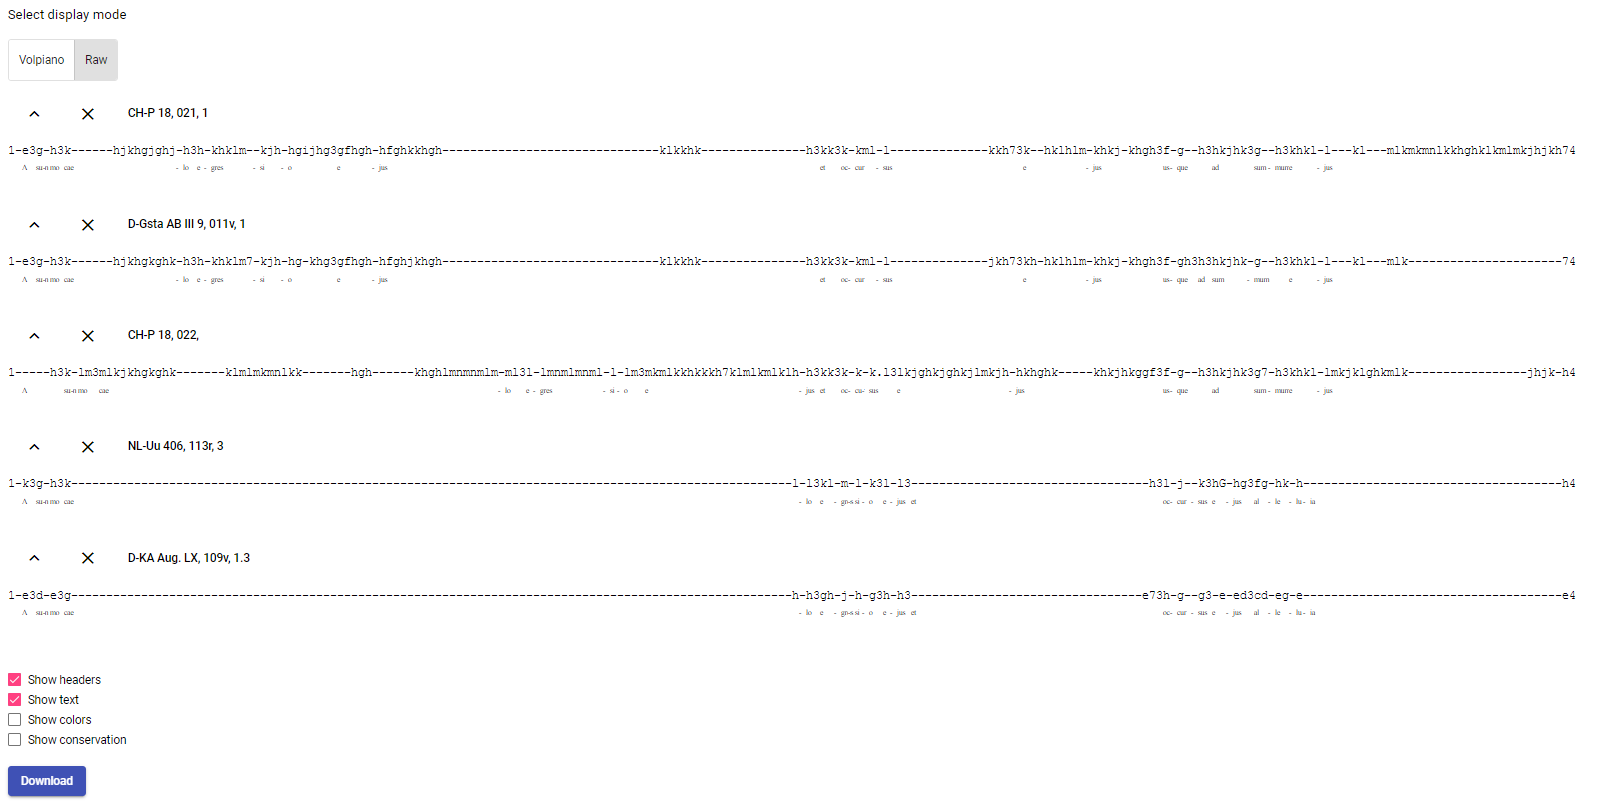
\includegraphics[scale=0.4]{udocs-alignment-raw}
\caption{Aligned melodies shown as the raw string.}
\label{fig:align-raw}
\end{figure}

To see the aligned sequences better, it is possible to remove the headers and the text independently by unclicking the corresponding boxes
in the alignment options (Figure \ref{fig:align-no-headers}, Figure \ref{fig:align-no-text}).

\begin{figure}[!h]
\centering
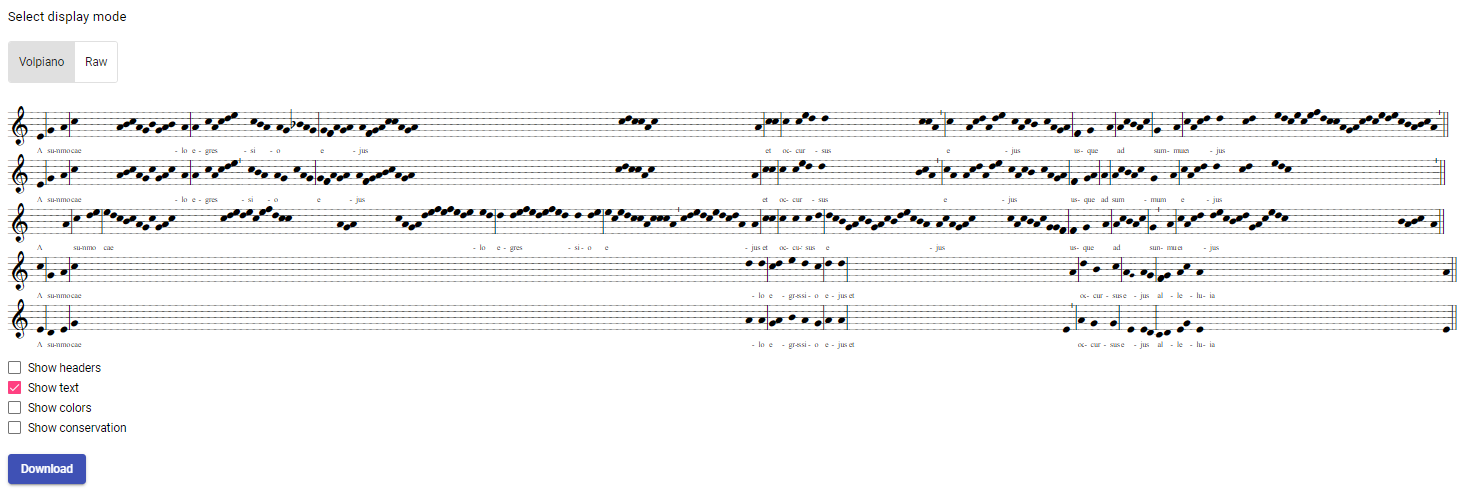
\includegraphics[scale=0.4]{udocs-alignment-no-headers}
\caption{The aligned melodies shown without headers.}
\label{fig:align-no-headers}
\end{figure}

\begin{figure}[!h]
\centering
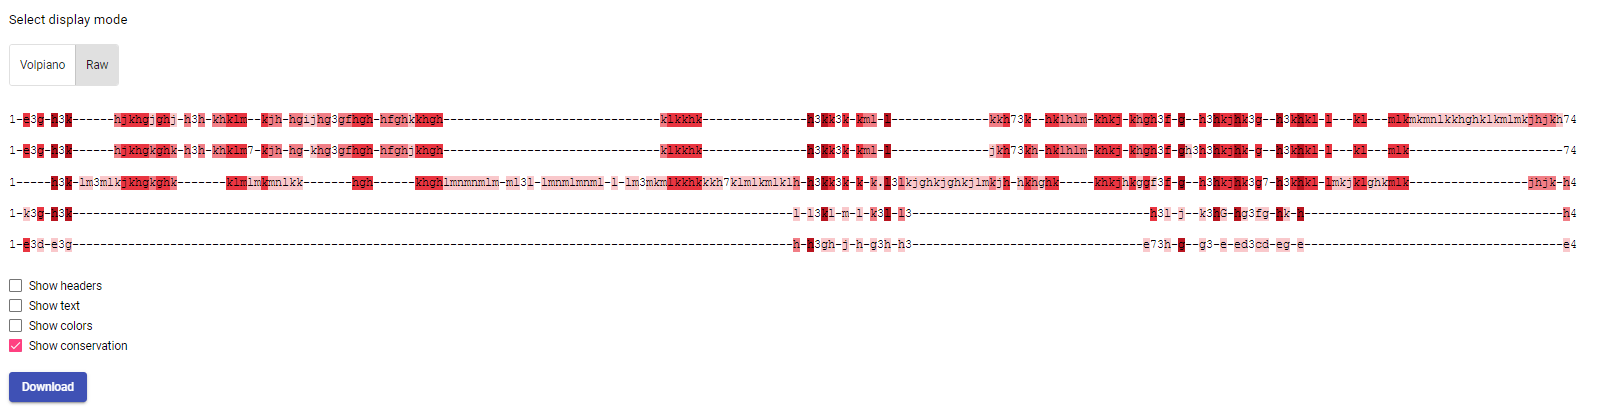
\includegraphics[scale=0.4]{udocs-alignment-no-headers-no-text}
\caption{The aligned melodies shown in \emph{Raw} mode without headers and text.}
\label{fig:align-no-text}
\end{figure}

It is possible to see how similar certain regions are. The first option is to color each note based on its absolute pitch (Figure \ref{fig:align-colors}).
In the case of interval alignment, this option may show different colors even though the intervals are the same.

\begin{figure}[!h]
\centering
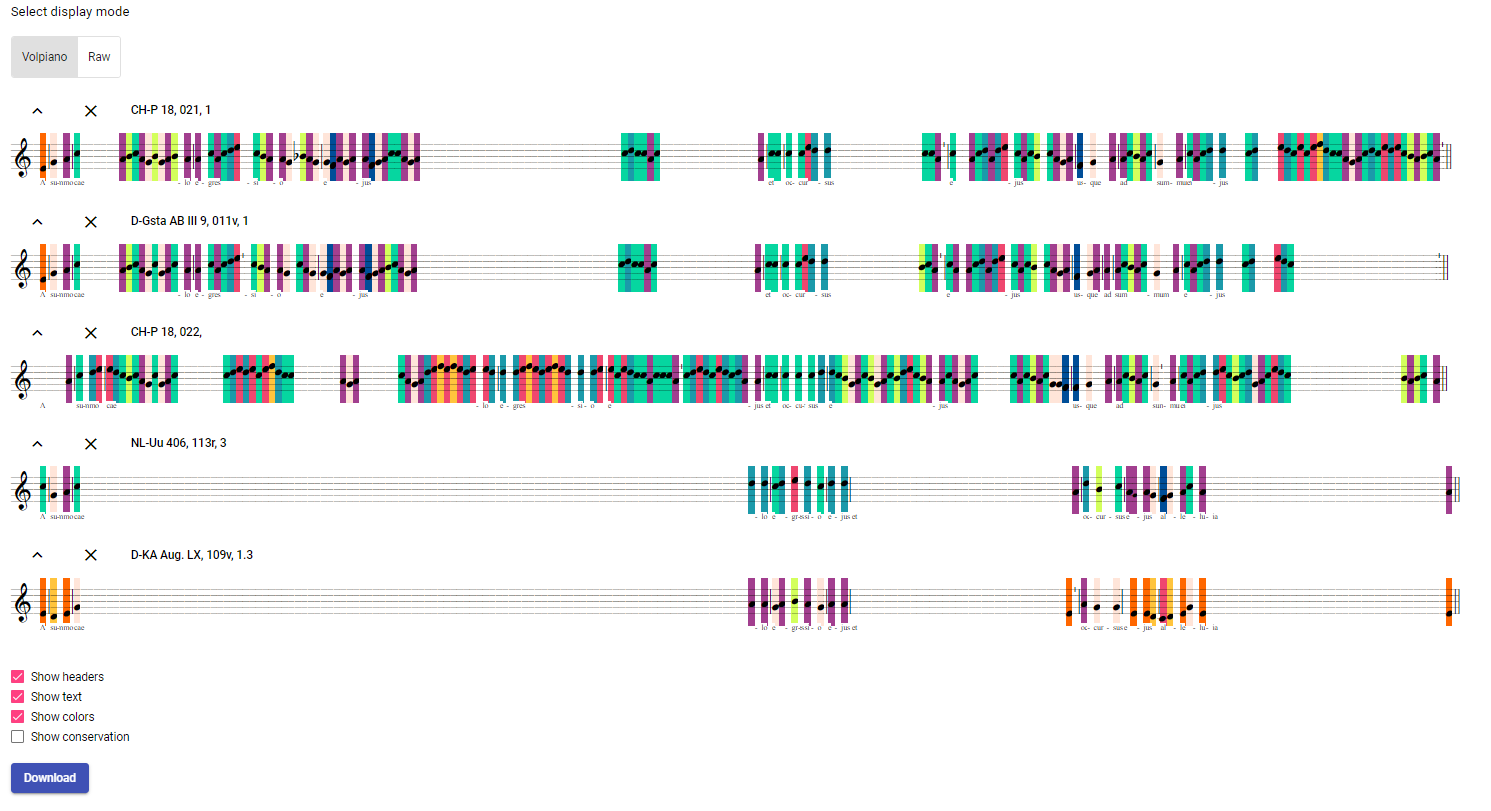
\includegraphics[scale=0.4]{udocs-alignment-vol-colors}
\caption{Aligned melodies with each note colored a different color.}
\label{fig:align-colors}
\end{figure}

The other option is to show the conservation profile, i.e. the proportion of the other chants sharing the same note or interval at the given position. This option will show
conservation profile corresponding to the intervals in the interval alignment option. Darker colors mean the position is more conserved, while lighter colors mean less conserved
(Figure \ref{fig:align-cons}). Moreover, this option shows the overall conservation indicator of the entire set.
Using this option, it is possible to see how similar entire regions are.

\begin{figure}[!h]
\centering
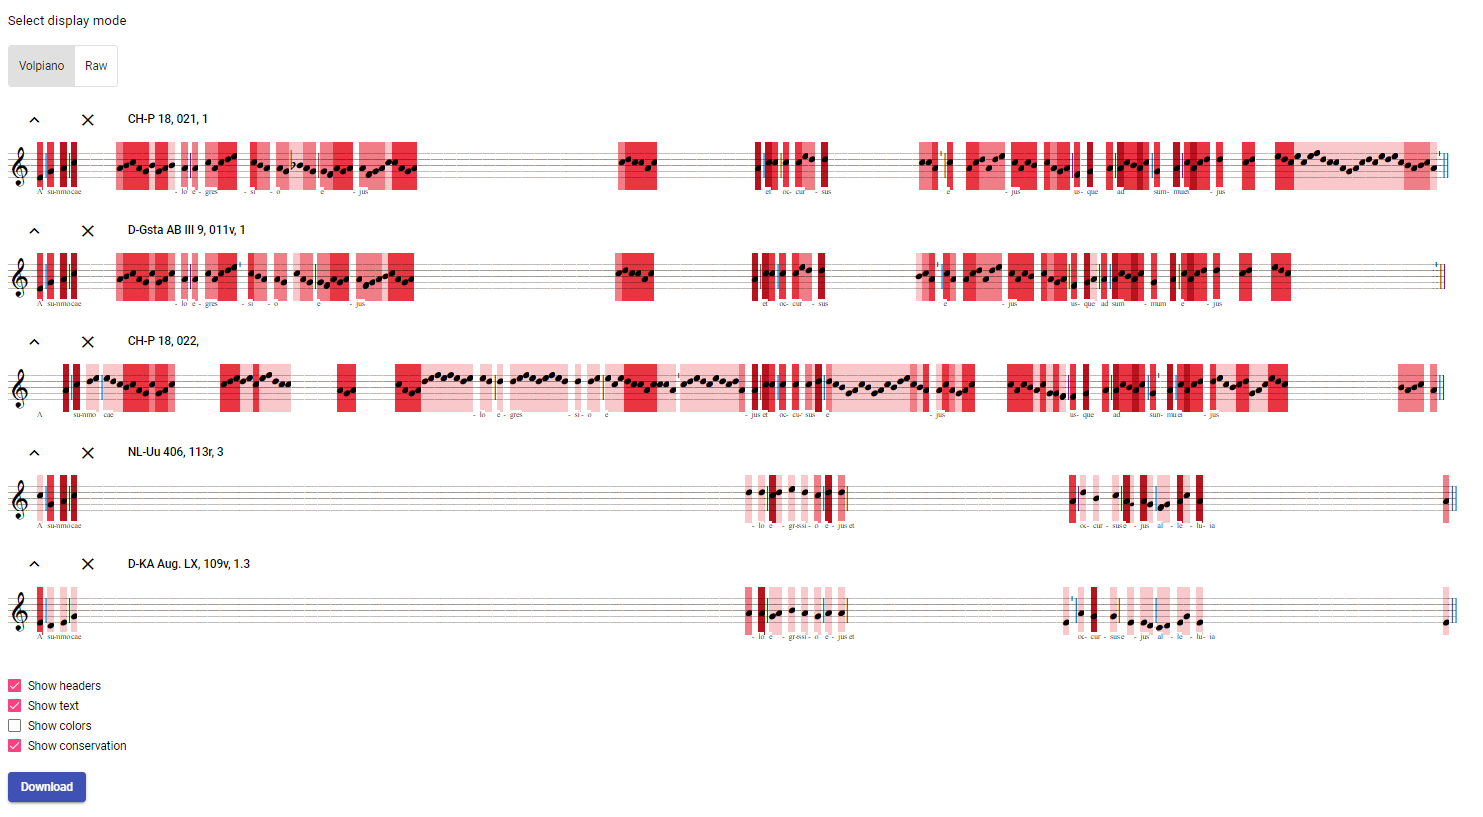
\includegraphics[scale=0.4]{udocs-alignment-vol-cons}
\caption{Aligned melodies with their conservation profile shown.}
\label{fig:align-cons}
\end{figure}

\subsection{Alignment export}

To export the aligned melodies, click the \emph{Download} button at the bottom of the page. The format of the file will be suitable to pass directly into MAFFT again. Each melody's
identifier is the string stored in the \emph{drupal\_path} field.

The melodies in the exported file will be either encoded as symbols corresponding to Volpiano characters in the case of naive and pitch alignment, or as symbols corresponding to intervals
in the case of interval alignment.

Only the unremoved melodies will be present in the file. Their order will be the same as the current order on the page.

\section{Dashboard}

The dashboard provides visualizations of the data. The visualizations are simple, as this feature is not the main priority of the application. Since at the time of development
it was not completely clear what data visualizations are useful for chant research, we only provide some most basic ones. Other visualizations will be added
as the application is used and it is clarified what researchers need most.

The dashboard is responsive, i.e. changing data sources has an immediate effect on the visualization.

The visualizations currently provided by the dashboard are comparison of melody length and text length for different data sources (Figure \ref{fig:dashboard1}),
a histogram of melody length (Figure \ref{fig:dashboard2}) and a histogram of text length (Figure \ref{fig:dashboard3}).

\begin{figure}[!h]
\centering
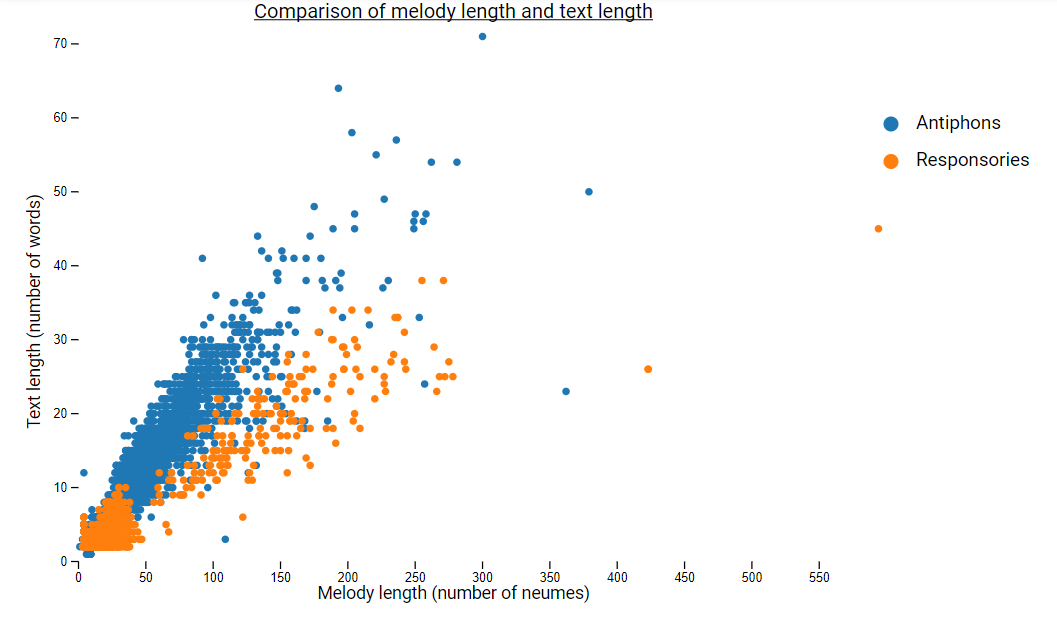
\includegraphics[scale=0.6]{udocs-dashboard-scatter}
\caption{Scatter plot of melody and text length for the data sources \emph{Antiphons} and \emph{Responsories}.}
\label{fig:dashboard1}
\end{figure}

\begin{figure}[!h]
\centering
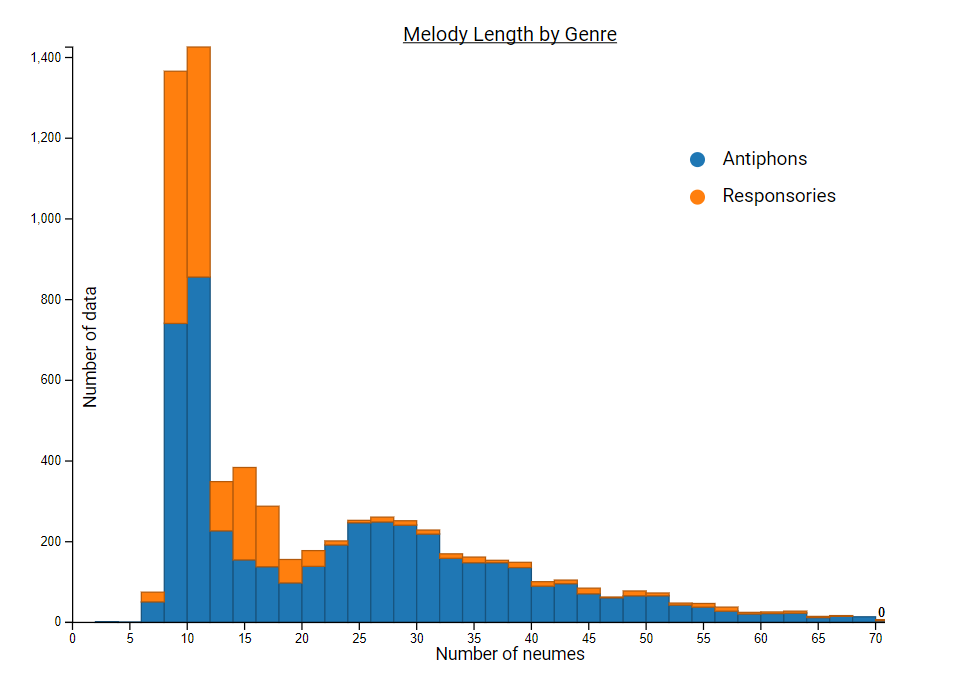
\includegraphics[scale=0.6]{udocs-dashboard-hist-melody}
\caption{Histogram of melody length for the data sources \emph{Antiphons} and \emph{Responsories}.}
\label{fig:dashboard2}
\end{figure}

\begin{figure}[!h]
\centering
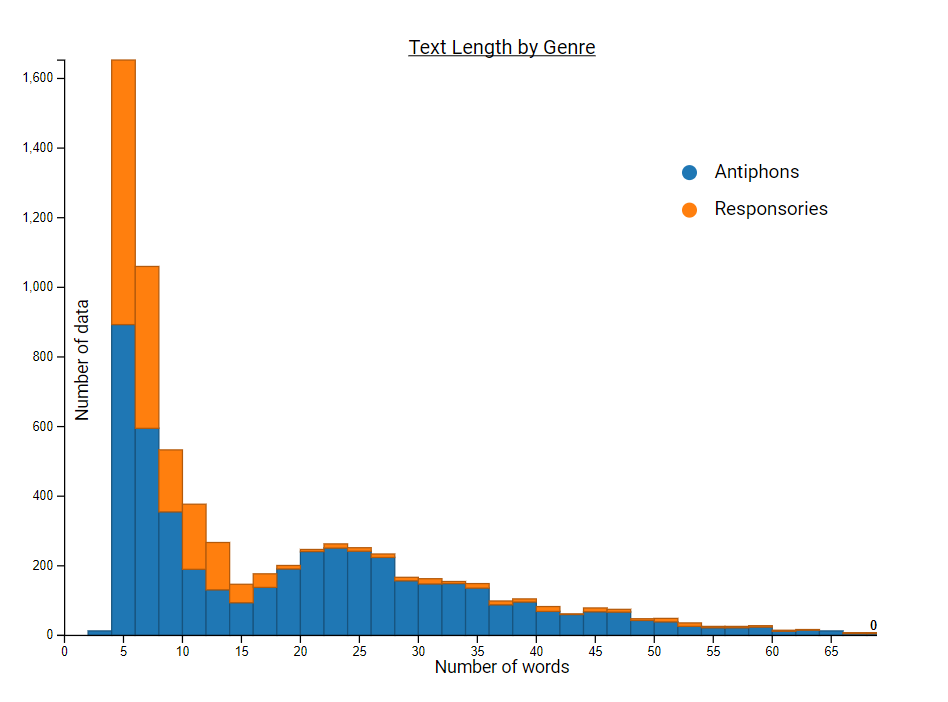
\includegraphics[scale=0.6]{udocs-dashboard-hist-text}
\caption{Histogram of text length for the data sources \emph{Antiphons} and \emph{Responsories}.}
\label{fig:dashboard3}
\end{figure}

\section{Known issues}

When displaying alignment results, some melodies may differ in their width on the screen even though they contain the same number of characters. This is caused by the font
Volpiano which does not have characters of equal width. There is no simple solution to this problem; to overcome it, we provide the option to display the alignment
as raw strings (not musical notation) using a monospaced font.

When aligning a larger number of chants (around 30 or more), the rendering becomes relatively slow and the page reacts to user input with a noticeable delay.
In the future, we may consider offering a simplified view without the interactive elements so that the delay is reduced to a minimum.

\chapter{Development documentation}

The software is a locally-run web application. It consists of three principal parts that ensure its proper functioning: the database, back end and
front end. Their interactions are outlined in Figure \ref{fig:architecture}.

\begin{figure}[!h]
\centering
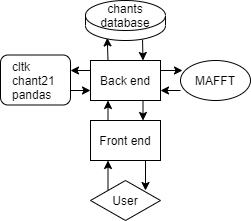
\includegraphics{ddocs_layout}
\caption{A high-level overview of the application's architecture.}
\label{fig:architecture}
\end{figure}

The database stores the data used by the application. The data it contains do not impact the functionality of the application. It can be added
to or removed from, as long as the added data follows the schema. It is even possible to have multiple databases and use the one that is currently needed.

The back end is the part of the application that takes care of the internal logic. It pulls data from the database and adds new ones. It performs calculations
that would be too compute-intensive for the front end. The back end is interacted with via its API: anyone can make an appropriate http request
to a specified URL and the back end returns the corresponding response.

The front end is the user-facing interface. Its main function is to display data returned by the back end. It can also perform some lighter calculations.
The user interacts with the front end via a web browser.

In the following sections, we will describe the proper functioning of each part in more detail.

\section{Data}

In this application, we use SQLite\footnote{\url{https://www.sqlite.org/}} as our data\-base technology. It is a lightweight and self-contained database engine,
which makes it easy to work with. It is the predefined database for the back end technology and comes with several drawbacks, such as a relatively low performance.
However, as our use case is not data-heavy, we have not opted for a different technology since we prefer flexibility over performance.

Our database consists of a single table \verb|chant|. The fields of one entry are described in Section \ref{section:db_fields}. Its schema is shown
in Figure \ref{fig:schema}.

\begin{figure}[!h]
\centering
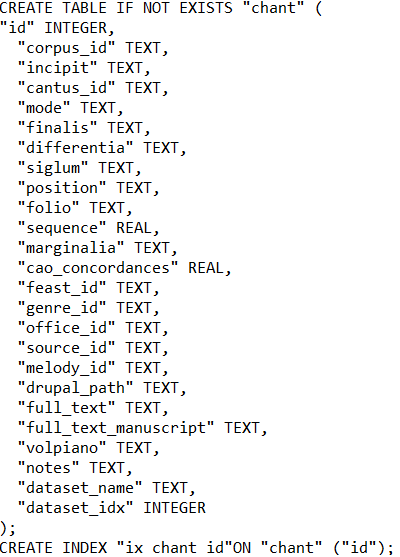
\includegraphics{ddocs_schema}
\caption{Schema of the \emph{chant} table.}
\label{fig:schema}
\end{figure}

The last two fields, \verb|dataset_name| and \verb|dataset_idx| determine to which data source the row belongs. Data source is the main grouping criterion
for data in this application. The user may select multiple data sources for comparison. The expected amount of data in each data source is in the order
of thousands of entries at most. We chose to store all data in one database, as opposed to e.g. having one database for each data source, as the expected
scale of data does not justify working with a more complex scheme.

\section{Back end}

The Python programming language is often used in academic contexts. It allows for rapid development and great flexibility. Python applications are easily
integrated with other programs, which we need for MAFFT integration. There are also many libraries available for working with data in general (e.g. \verb|pandas|)
and for our specific data (\verb|cltk| for working with Latin texts, \verb|chant21| for working with chants). Because of these properties, we decided to use Python
for our application's back end.

The back end uses the Django framework.\footnote{\url{https://www.djangoproject.com/}} Django is a Python web framework enabling developers to create web
applications quickly, having abstracted away the most tedious of web development aspects.

Django programs consist of one or more logical units called \emph{apps}. An \emph{app} is a self-contained program providing some related functionality. Thanks
to Django's modularity, an \emph{app} can be plugged in into many projects without the need to always rewrite it. Our application only uses one \emph{app},
\verb|melodies|, which provides REST API to other programs.

% the app only contains one app, melodies
The app only contains one app, \verb|melodies|, which provides the API for other applications. The app uses the module \verb|core| providing the essential
computations.

To ensure proper integration with the front end, it is necessary to include allow front end's server to interact with the back end. This is done by
including front end's URL in the array \verb|CORS_ORIGIN_WHITELIST| in the \verb|settings.py| file. In the event of deployment, the URL
would need to be changed appropriately.

\subsection{REST API}
\label{section:api}

The \verb|melodies| app provides API that offers other programs a way of interacting with it. It is done in the form of web requests to a specific URL. The requests
can be either GET or POST requests. GET requests do not contain any additional data; the response returned always depends only on the state of the application. On
the contrary, POST requests contain data that the application takes into account when constructing the response.

Table \ref{table:api} summarizes the API provided by the application. The API is described into more detail below.

\begin{longtable}{| p{.24\textwidth} | p{.09\textwidth} | p{.18\textwidth} | p{.39\textwidth} |} 
%\begin{center}
%\begin{tabular}{| c | c | c | c |} 

 \hline
 Endpoint & Method & POST fields & Description \\
 \hline
\emph{api/chants/}                & POST & \verb|dataSources|, \verb|incipit|, \verb|genres|, \verb|offices| & Returns a list of chants filtered by their data source, incipit, genre and office\\
\emph{api/chants/\textless pk\textgreater} & GET  &                                                          & Returns the chant with the ID \verb|<pk>|\\
\emph{api/chants/sources}         & GET  &                                                                   & Returns a list of all data sources currently present in the database with their name and index\\
\emph{api/chants/upload/}         & POST & \verb|file|, \verb|name|                                          & Uploads \verb|file| to the database as a new data source and gives it the specified \verb|name|\\
\emph{api/chants/export/}         & POST & \verb|idsToExport|                                                & Returns a CSV file containing the chants with the specified IDs\\
\emph{api/chants/create-dataset/} & POST & \verb|idsToExport|, \verb|name|                                   & Creates a new data source from the chants with the specified IDs and gives it the specified \verb|name|\\
\emph{api/chants/align/}          & POST & \verb|idsToAlign|, \verb|mode|                                    & Takes chants with the specified IDs and aligns them according to \verb|mode|\\
 \hline

%\end{tabular}
%\end{center}
\caption{API of back end.}
\label{table:api}
\end{longtable}

\begin{itemize}

\item \textbf{api/chants/} The POST request must contain the fields as specified in Table \ref{table:api}. \verb|dataSources| is a list of indices of allowed data sources as stored
in the database. \verb|incipit| is a string that must be present as a substring in the \emph{incipit} field in each of the returned entries. \verb|genres| and \verb|offices|
are lists of strings, where each string is an identifier of a genre or an office, as seen in Attachment XX. Each returned entry must have its genre be an element of \verb|genres|
and its office be an element of \verb|offices|. The response is a list of all entries in the database satisfying these constraints.

\item \textbf{api/chants/\textless pk\textgreater} The application looks for a chant with the ID \verb|pk| in the database. It returns an error if no such entry exists. If it does,
it returns a JSON object with the following keys: \emph{db\_source}, which is the entry as stored in the database, \emph{json\_volpiano}, which is the chant processed in
such a way that its melody and text are easy to display in an HTML template, and \emph{stresses}, a list of stressed syllables corresponding to the chant's text, if it
can be computed.

\item \textbf{api/chants/sources} The response is a JSON object with one key, \verb|sources|. Its value is the list of pairs representing the data sources currently present in
the database. The first value of each pair is a data source index and the second one is its name.

\item \textbf{api/chants/upload/} The POST request must contain a CSV file as specified in Section XX in the field \verb|file| and a string \verb|name|. The data in the file
will be uploaded directly to the database as a new data source with the given name. Some values may be changed before inserting the data in the database, namely the columns
\emph{id}, \emph{dataset\_idx}, and \emph{dataset\_name}, if the file contains them. The response is a JSON object with the keys \emph{name}, the name of the new data
source, and \emph{index}, the index assigned to it.

\item \textbf{api/chants/export/} The POST request body must contain the field \verb|idsToExport|. It is a list of integers representing the IDs of the chants to be exported. If
an ID does not correspond to any chant in the database, the ID will be excluded. The response contains a CSV file with its entries being the corresponding chants, formatted
as outlined in Section XX.

\item \textbf{api/chants/create-dataset/} The POST request must contain a list of chant IDs in the field \verb|idsToExport| and a string in the field \verb|name|. The chants
that correspond to the IDs will be duplicated in the database, given new IDs and assigned to a new data source with the name as specified in the field \verb|name|.
The response is the same JSON object as in the \emph{upload} API, containing the keys \emph{name} and \emph{index}, the name and index of the newly created data source.

\item \textbf{api/chants/align/} The POST request contains two fields. \verb|idsToAlign| is the list of chant IDs we want to align. \verb|mode| is the mode of alignment we chose.
Its values can be \emph{syllables}, which is the word-based alignment, \emph{full}, the alignment on pitches, or \emph{intervals}, the alignment on intervals. If the
value is not one of those, the request will return an error. The response is a JSON object with the following keys: \emph{chants} is an object representing the
aligned melodies along with their texts, easily renderable by an HTML template. \emph{errors} contains a list of chant IDs of the chants that could not be aligned for
various reasons. \emph{successes} contains an object that describes the chants that have been successfully aligned: \emph{sources} are their original sources (i.e.
siglum, folio and position), \emph{ids} the IDs as stored in the database, \emph{volpianos} the melodies as given by the alignment algorithm, and \emph{urls} the
values in the \emph{drupal\_path} field of the database.

\end{itemize}

\subsection{Core}

\verb|core| is the Python module that contains essential functionality ensuring the proper behavior of the application, e.g. the implementation of alignment,
MAFFT integration, and others. Figure \ref{fig:core} outlines the classes provided in the submodule and how they interact. The classes' functionality
is described below.

% MAFFt dat mimo core
% farebny hranaty ramcek pre core
% mozno aj napisat cltk
% prehodit api a core sekcie - a rovno napisat ktore api calls to pouzivaju
\begin{figure}[!h]
\centering
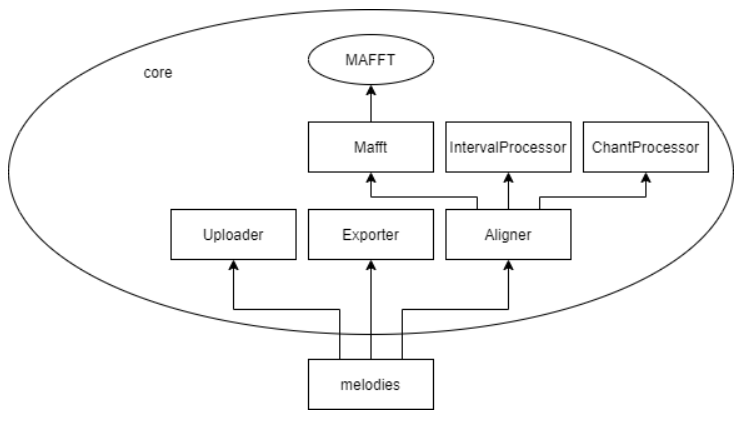
\includegraphics[scale=0.9]{ddocs_core}
\caption{Outline of the classes contained in \emph{core} and their interaction. An arrow from A to B indicates that A depends on B.}
\label{fig:core}
\end{figure}

% vyraznejsie nadpisy pre triedy - napr subsubsection
\begin{itemize}

\item\textbf{Exporter.} The class contains one method, \verb|export_to_csv|. It takes as an argument a list of chant IDs contained in the database. It returns
a response with a file with the corresponding database entries formatted as CSV.

\item\textbf{Uploader.} The class defines one method, \verb|upload_csv|. Its arguments are a \emph{pandas}\footnote{\url{https://pandas.pydata.org/}} dataframe, containing
data columns as described in Section \ref{section:db_fields}, and a dataset name. The method inserts the data into the database, ensuring that no duplication 
of IDs occurs. Input sanitization is done by the Django framework.

\item\textbf{ChantProcessor.} The class contains functionality for working with Latin texts and with melodies encoded as Volpiano. The method \verb|get_syllables_from_text|
takes a string of Latin text and returns the text syllabified: the returned value is a list, each of whose elements represents a word of the text, and each word
is a list of strings representing the syllables in that word. To syllabify the text, we use the module \verb|cltk|,\footnote{\url{http://cltk.org/}} which facilitates
working with classical languages, including Latin.

Some parts of the application require the encoded melody to contain no \verb|-| characters. Instead, they assume that ends of words are marked with a tilde (\verb|~|) and ends of
syllables with a pipe (\verb=|=). The method that converts proper Volpiano-encoded melody to this processed format is the method \verb|insert_separator_chars|.
The equivalent of syllabifying text for melodies is \verb|get_syllables_from_volpiano|. It takes a melody encoded as a processed Volpiano string (with \verb|~| and \verb=|=
instead of \verb|-|.). It assumes that the
melody contains a clef at the first position and a bar line at the last position, which is the proper way of encoding melodies according to the Volpiano
protocols.\footnote{\url{https://cantus.uwaterloo.ca/sites/default/files/documents/2.\%20Volpiano\%20Protocols.pdf}} The method returns a list whose elements represent words,
and each word is a list of strings representing syllables (equivalent to the syllabifying method for text). Examples of using these functions are shown in Figure \ref{fig:syl_text}
and Figure \ref{fig:syl_volpiano}.

\begin{figure}[!h]
\centering
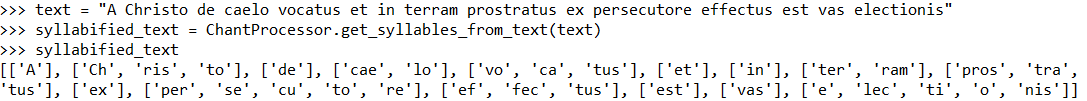
\includegraphics[scale=0.6]{ddocs_text-to-syllables}
\caption{Example of dividing Latin text into syllables using \emph{ChantProcessor}.}
\label{fig:syl_text}
\end{figure}

\begin{figure}[!h]
\centering
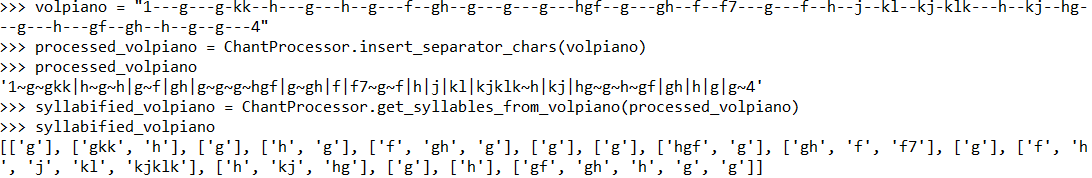
\includegraphics[scale=0.6]{ddocs_volpiano_to_syllables}
\caption{Example of dividing a melody encoded as Volpiano into syllables using \emph{ChantProcessor}.}
\label{fig:syl_volpiano}
\end{figure}

The method \verb|get_stressed_syllables| takes a Latin string as input and returns a list whose elements represent words, where word is a list of 0s and 1s,
a 0 representing an unstresed syllable and a 1 representing a stressed one. To calculate the stressed syllables, we use the module \verb|cltk|. However, 
its stress recognition is not completely accurate, therefore this method may also return incorrect results. However, no other functionality depends on
the results of the stress calculation. The function is shown in use in Figure \ref{fig:syl_stress}.

\begin{figure}[!h]
\centering
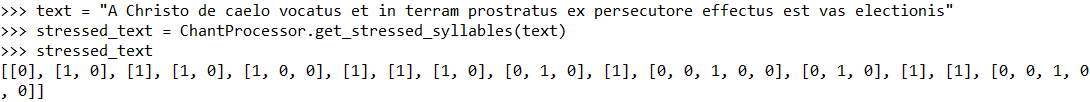
\includegraphics[scale=0.6]{ddocs_syllables-stressed}
\caption{Example of finding the stressed syllables of a Latin text using \emph{ChantProcessor}.}
\label{fig:syl_stress}
\end{figure}

\item\textbf{IntervalProcessor.} The class provides tools to work with the interval representation of a melody. It contains two methods, \verb|transform_volpiano_to_intervals|
and \verb|transform_intervals_to_volpiano|. \verb|transform_volpiano_to_intervals| takes a string representing a melody (it can be encoded either as dictated by the Volpiano protocol, or processed
to have its words separated by \verb|~|s and syllables by \verb=|=s for the purposes of alignment, see Section \ref{section:vol_preprocess}) and returns the same melody represented as intervals.
\verb|transform_intervals_to_volpiano| is its reverse: it takes a string representing a melody encoded by intervals and returns the Volpiano representation.
Figure \ref{fig:vol_intervals} shows how these functions are used.

\begin{figure}[!h]
\centering
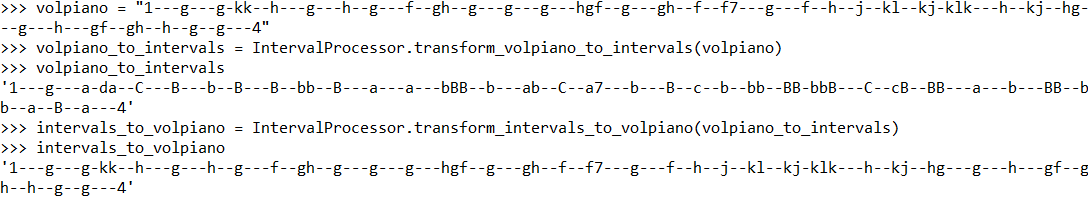
\includegraphics[scale=0.6]{ddocs_intervals}
\caption{Transforming a Volpiano-encoded melody into an interval representation and back.}
\label{fig:vol_intervals}
\end{figure}

\item\textbf{Mafft.} This class provides the interface for working with the MAFFT software.\footnote{\url{https://mafft.cbrc.jp/alignment/software/}} The software must be installed
on the computer that runs the application. On Windows systems, it is assumed that it is installed in a WSL instance.\footnote{\url{https://docs.microsoft.com/en-us/windows/wsl/}}
On other systems, it has to be installed natively.

An instance of the class encapsulates the action of aligning one set of data. It needs to have a specified input file, and, optionally, an output file, which can be set
via the methods \verb|set_input| and \verb|set_output|. If the user wishes to run the alignment with other options as specified in MAFFT's documentation, it can be done
using the method \verb|add_option|. The method \verb|add_volpiano| can optionally be used if the user does not want to provide their own file (however, its location must
still be defined) or wishes to add another sequence to align. MAFFT is only run by calling \verb|run_process|. The result of the alignment is retrieved using the methods
\verb|get_aligned_sequences| and \verb|get_sequence_order|, which return the aligned sequences and their headers, respectively, in the order of similarity.

\item\textbf{Aligner.} The class defines the methods to compute the three types of alignment, as described in Section \ref{section:chant_alignment}: \verb|alignment_syllables|,
which performs the word-based alignment; \verb|alignment_pitches|, computing the alignment of pitches; and \verb|alignment_intervals|, which return the alignment of 
intervals. All of them take as an argument just the list of IDs of the chants to be aligned and return a dictionary easy to work with in HTML templates.
% alignment_syllables nepouziva triedu mafft, ostatne ano - interval pouziva aj interval processor

\end{itemize}

\section{Front end}

For the front end, our application uses the Angular framework.\footnote{https://angular.io/} An Angular application
consists of components, which are small, relatively self-contained units exposing some functionality of the application (both appearance and behavior), and
services, providing means of sharing and manipulating data, e.g. the interaction with the back end. Both components and services should only contain
a small, logically contained set of functionality. This makes the application safe and scalable. Most importantly, the framework keeps track of the data
passed to it and updates the appearance dynamically.

This application contains several components and services that interact with each other. Figure \ref{fig:frontend-schema} shows a diagram of the front end architecture.
The elements in rectangles are components. Orange background, \emph{AppComponent}, represents the component encapsulating the entire application. Blue
background represents components that are always present on the page. A dotted arrow from component A to component B indicates that component A has component
B in its HTML template. The ellipses represent services. An arrow from a component or service A to service B means that element A uses service B.

The following sections describe each service and component in more detail.

% pridat do popisku co su obdlzniky etc
% vyfarbit podla toho na ktorej su stranke
% hruba farebna sipka "api calls"
\begin{figure}[!h]
\centering
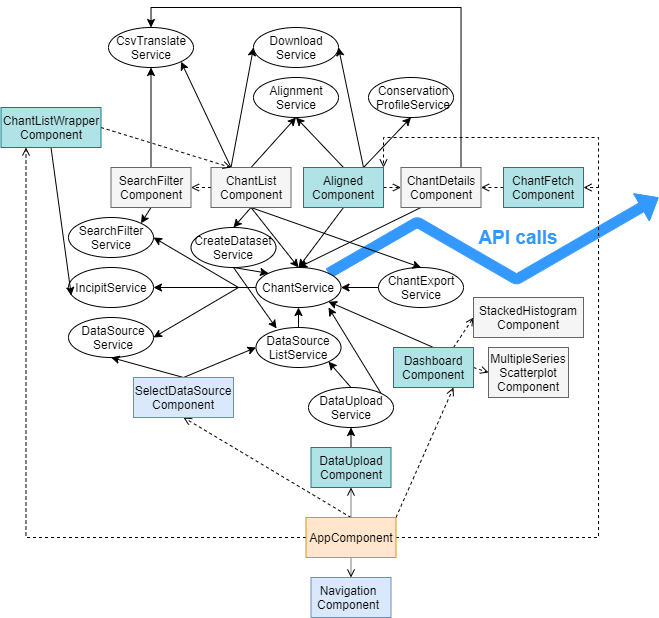
\includegraphics[scale=0.8]{ddocs_frontend-schema}
\caption{The architecture of the front end.}
\label{fig:frontend-schema}
\end{figure}

\subsection{Services}

% urobit z toho zoznam

\begin{itemize}

\item\textbf{ChantService.} This service is the service responsible for communication with the back end. It uses back end's API as described in Section \ref{section:api} to
obtain the desired data. The method \verb|getChant|, taking a single number as an argument, sends a request to the back end to retrieve the chant with 
the ID equal to the argument. The method \verb|loadData| uses the current values stored int \emph{IncipitService}, \emph{SearchFilterService}, and
\emph{DataSourceService} to obtain all chants adhering to the constraints; the method \verb|getList| provides the object where these results are stored.
The method \verb|getAlignment| takes a list of chant IDs and an alignment mode and makes a request to the back end to calculate the corresponding alignment.
\verb|getDataSources| obtains all data sources currently present in the database. \verb|exportChants| takes as an argument a list of chant IDs and the 
corresponding API call returns a CSV file with their database entries. \verb|createDataset| creates a new data source from the chant IDs and name provided
to it. All arguments to these functions are passed as a part of a \emph{FormData}\footnote{https://developer.mozilla.org/en-US/docs/Web/API/FormData}
object.

\item\textbf{IncipitService.} The service stores the value of the incipit search query which is used when pulling data from the database. It provides two methods:
\verb|setIncipit| which changes the current value of the search query, and \verb|incipit| which returns a \emph{BehaviorSubject}\footnote{https://www.learnrxjs.io/learn-rxjs/subjects/behaviorsubject}
storing the value.

\item\textbf{SearchFilterService.} The service stores an object containing a list of allowed genres and a list of allowed offices which will be used for filtering
when retrieving data from the database. It provides two methods, \verb|setFilterSettings|, which changes the current value, and \verb|getFilterSettings|, returning
a \emph{BehaviorSubject} with the value.

\item\textbf{DataSourceService.} The service stores a list of indices of data sources we are currently using. The stored value persists throughout browser sessions.
The service has two methods, \verb|setSourceList|, which changes the value, and \verb|getSourceList|, which returns a \emph{BehaviorSubject} with the list.

\item\textbf{DataSourceListService.} The service stores a list of the data sources in the database as of the time of the last call to the back end's API. The list
is accessed by calling \verb|getAllSources|. The method \verb|refreshSources| retrieves the current list of data sources from back end.

\item\textbf{CreateDatasetService.} The service contains one method, \verb|createDataset|. It takes as an argument a list of chant IDs and a data source name and
ensures that it is sent to back end to be inserted into the database. Additionally, it calls \emph{DataSourceListService}'s \verb|refreshSources| to obtain the
most recent list of data sources.

\item\textbf{DataUploadService.} The service contains one method, \verb|uploadData|. It takes two arguments, a CSV file and a data source name. It passes these to \emph{ChantService}
to be inserted into the database and assures that the current data source list is correct by a call to \emph{DataSourceListService}.

\item\textbf{ChantExportService.} The service provides one method, \verb|exportChants|. Its argument is a list of chant IDs to be exported. The method returns a CSV
file with these chants.

\item\textbf{CsvTranslateService.} The service provides means to obtain a genre's or an office's full description given its identifier as stored in the database.
The descriptions are sourced from CSV files provided in CantusCorpus. They can be accessed via the methods \verb|getGenre| and \verb|getOffice|, both
taking the identifier of the genre or office as an argument. The service also contains the method \verb|getAllValues|, which takes as an argument either
the string \emph{genres} or \emph{offices}, and returns an object containing all values of the given type.

\item\textbf{DownloadService.} The service contains a single method, \verb|download|. It takes two arguments: \verb|blob|, which is the content of a file to
be downloaded, and \verb|filename|, the name of the file. Calling the method triggers the download of the file. The service is used in multiple situations.
It ensures the download of CSV files with exported chants, as well as the download of text files with the results of the alignment.

\item\textbf{AlignmentService.} The service stores the IDs of chants we want aligned and the algorithm using which they should be aligned. Both of these values persist
throughout browser sessions. The IDs can be changed or obtained by calling the setter and getter on \verb|idsToAlign|. The algorithm can be set via the method
\verb|setMode|, which returns 0 if the provided algorithm is correct and 1 otherwise; and retrieved with the method \verb|getMode|. The allowed algorithm values are
\emph{full}, \emph{intervals}, and \emph{syllables.}

\item\textbf{ConservationProfileService.} The service contains only one method called \verb|calculateConservationProfile|. Given a list of aligned melodies, as computed by the back end,
it calculates the conservation value for each position in each melody. It returns it in a form easy to work with in HTML templates.

\end{itemize}

\subsection{Components}

% screenshoty - moze byt viac komponentov v jednom komponente

\begin{itemize}

\item\textbf{AppComponent.} This component is the one always present on the page, encapsulating other components. It defines the global styles of the entire page.
The component displays \emph{SelectDataSourceComponent} and \emph{NavigationComponent}, which means they are always visible on the page. It further displays
components depending on the current URL, as indicated by the \verb|router-outlet| tag.

\item\textbf{NavigationComponent.} The component provides easy navigation to the app's main pages. It also enables the user to enter a query for searching
among the chants' incipits via the field in the top right corner. The \emph{home} button in the top left corner leads to the landing page.

\item\textbf{SelectDataSourceComponent.} The component exposes the interface to change the current selection of data sources. It contains a list of data sources
names, each next to a checkbox. The \emph{Save} button saves the current selection of data sources.

\item\textbf{ChantLlistWrapperComponent.} The component encapsulates \emph{ChantListComponent}. It reads the incipit search query from the current URL and
passes it to \emph{IncipitService}.

\item\textbf{ChantListComponent.} The component displays a list of chants from the current search results. The table contains a chant's incipit, source, genre, office, and
its data source. The checkboxes next to the incipits allow for the chants' selection. The component also provides the possibility to filter search
results, to export a selection of chants, to align a selection, and to create a new data source.

\item\textbf{SearchFilterComponent.} The component enables the user to select which genres and offices should be included in search results. It consists of
a set of checkboxes that determine whether a specific genre or office is allowed or not. The settings are saved using the \emph{Save} button.

\item\textbf{AlignedComponent.} The component displays results of alignment. It shows the aligned chants ordered by similarity in rows under each other. It
provides the means to hide and unhide text and headers, completely remove or collapse an alignment, rearrange the order, as well as highlight notes and
conservation profile. It also provides the possibility to export the results to a file.

\item\textbf{ChantFetchComponent.} The component encapsulates \emph{ChantDetailsComponent}. It reads chant ID from URL and passes it to \emph{ChantDetailsComponent}.

\item\textbf{ChantDetailsComponent.} The component displays the relevant information about a selected chant. It displays a melody with its text whose stressed
syllables are highlighted if possible.

\item\textbf{DashboardComponent.} The component displays several visualization of data from the current search selection. It preprocesses the data sent to
each of the visualizations.

\item\textbf{StackedHistogramComponent.} The component contains a histogram of data passed to it. We use the library \emph{d3js}\footnote{\url{https://d3js.org/}}
for the plot creation.

\item\textbf{MultipleSeriesScatterplotComponent.} The component shows a scatter plot of data passed to it. Again, we use the library \emph{d3js}.

\item\textbf{DataUploadComponent.} The component displays the interface for uploading a file to the database.

\end{itemize}

\section{Dependencies}

The software depends on several other programs for its correct functionality. For the back end, it is necessary to have Python installed. During development,
version 3.9.2 was used; it is not guaranteed that the application will work for lower versions. Additionally, the packages Django (version 3.1.7), pandas (version 1.2.3)
chant21 (version 0.4.6) and cltk (version 1.0.5) are required. It is also necessary to have the MAFFT software installed (version 7.470 or higher).

The front end is run on Angular version 11. It uses the library d3 (version 7.6.0) for visualizations.



\chapter*{Conclusion}
\addcontentsline{toc}{chapter}{Conclusion}

The outcome of this thesis is an interdisciplinary software tool applying methods from bioinformatics to digital musicology, enabling researchers
to analyze relatively large amounts of data computationally. The software
provides the ability to investigate the origin and evolution of a set of chants. An important implication of this ability is that it facilitates
the discovery of contrafacta (chants with different lyrics but the same melodies) and transpositions (chants whose melodies differ by an interval
in all positions), which is a task that lacked the proper tools until now.

To analyze the chants, we used techniques from bioinformatics, namely multiple sequence alignment algorithms. These techniques have been used by
biologists for a long time to study the same properties - origin and evolution - of biological sequences. As chant melodies and biological sequences
share many properties, and, importantly, MSA algorithms do not require assumptions about chants that we cannot guarantee, these methods are suitable
for studying Gregorian chant.

Our work bridges the gap between traditional musicology,
which relied on the individual ability to draw conclusions from analog sources, and computational analysis. The software is a tool
that will have immediate applications in the basic research of Gregorian chant, such as the study of \emph{Jistebnice Cantionale}.\footnote{
Done in collaboration with the \emph{Old Myths, new Facts} project at the Masaryk Institute of the Czech Academy of Sciences and the Faculty
of Arts of Charles Univeristy.}

Originally, one of the purposes of this work was to create a set of visualizations that would facilitate the quantitative analysis of a set of chants.
However, during the development process it became clear that musicology itself has not yet formalized many of its problems in such a way that 
would make it clear what types of quantitative analysis is actually needed.\footnote{From personal communication with Dr. Jennifer Bain and Dr.
Debra Lacoste.} In fact, the alignment tool proved to be much more useful for immediate
applications\footnote{From personal communication with doc. PhDr. Hana Vlhová-Wörner, Ph.D}. Therefore, our attention shifted to the proper
development of the alignment tool. The visualization part is left for further development, in hopes that the desired use cases crystallize into
a more definite form in the future.

The software continues to be developed in collaboration with the Czech Aca\-demy of Sciences.

\section*{Future work}

Computing multiple sequence alignment opens the door to many other applications. Our software touches upon one
of them by providing the ability to calculate the conservation profile; thhe natural next step is to use the results of the alignment to
obtain and visualize the phylogenetic tree of the set, i.e. their
``family tree'' showing how the individual melodies changed and developed. The tree's visualization could make it easier to see
the relationship between the melodies without the need to study the alignment.

Another possibility is to use the similarity matrix obtained from the alignment to visualize a network of the chants. The clusters
forming in this visualization could show related groups of chants and reveal relationships that were not obvious before.

The opportunities promised by MSA algorithms are vast. We plan to explore more of those that will be determined to be useful for the study of Gregorian
chant, as we continue with the development of the software in collaboration with chant researchers, and we are looking forward to new discoveries.


%%% Bibliography
%%% Bibliography (literature used as a source)
%%%
%%% We employ bibTeX to construct the bibliography. It processes
%%% citations in the text (e.g., the \cite{...} macro) and looks up
%%% relevant entries in the bibliography.bib file.
%%%
%%% The \bibliographystyle command selects, which style will be used
%%% for references from the text. The argument in curly brackets is
%%% the name of the corresponding style file (*.bst). Both styles
%%% mentioned in this template are included in LaTeX distributions.

\bibliographystyle{plainnat}    %% Author (year)
% \bibliographystyle{unsrt}     %% [number]

\renewcommand{\bibname}{Bibliography}

%%% Generate the bibliography. Beware that if you cited no works,
%%% the empty list will be omitted completely.

\bibliography{bibliography}

%%% If case you prefer to write the bibliography manually (without bibTeX),
%%% you can use the following. Please follow the ISO 690 standard and
%%% citation conventions of your field of research.

% \begin{thebibliography}{99}
%
% \bibitem{lamport94}
%   {\sc Lamport,} Leslie.
%   \emph{\LaTeX: A Document Preparation System}.
%   2nd edition.
%   Massachusetts: Addison Wesley, 1994.
%   ISBN 0-201-52983-1.
%
% \end{thebibliography}


%%% Figures used in the thesis (consider if this is needed)
\listoffigures

%%% Tables used in the thesis (consider if this is needed)
%%% In mathematical theses, it could be better to move the list of tables to the beginning of the thesis.
\listoftables

%%% Abbreviations used in the thesis, if any, including their explanation
%%% In mathematical theses, it could be better to move the list of abbreviations to the beginning of the thesis.
\chapwithtoc{List of Abbreviations}

%%% Attachments to the bachelor thesis, if any. Each attachment must be
%%% referred to at least once from the text of the thesis. Attachments
%%% are numbered.
%%%
%%% The printed version should preferably contain attachments, which can be
%%% read (additional tables and charts, supplementary text, examples of
%%% program output, etc.). The electronic version is more suited for attachments
%%% which will likely be used in an electronic form rather than read (program
%%% source code, data files, interactive charts, etc.). Electronic attachments
%%% should be uploaded to SIS and optionally also included in the thesis on a~CD/DVD.
%%% Allowed file formats are specified in provision of the rector no. 72/2017.
\appendix
\chapter{Attachments}

\section{First Attachment}

\openright
\end{document}
